%% Hello emacs, this is -*- latex -*-
\typeout{ ====================================================================}
\typeout{ This is file neural.tex, created at 27-Aug-2005 }
\typeout{ Maintained by Andre Anjos <Andre.dos.Anjos@cern.ch> }
\typeout{ ====================================================================}

\chapter{Análise neural baseada em calorimetria para a deteção
elétron/jato} 
\label{chap:neural}

Neste capítulo desenvolvem-se sistemas de classificação de simples treinamento
e emprego, baseados em redes neurais artificais. Estes classificadores definem
um patamar de deteção melhor que o sistema discutido no capítulo anterior,
superando-o em robustez e flexibilidade e ainda atingindo uma velocidade de
execução compatível com a operação dentro do Segundo Nível do Sistema de
Filtragem do experimento ATLAS.

\section{Revisão da literatura}
\label{sec:review}

Dentre os métodos modernos de análise multi-variável mais empregados em Física
de Altas Energia, Redes Neurais Artificiais possuem um papel importante ao
lado de outras técnicas também eficazes como a Análise de Componentes
Principais e classificadores bayesianos. Nesta seção conduz-se uma revisão
literária deste tipo de análise, empregada atualmente neste campo da física.

Os primeiros sistemas de deteção baseados em análise neural, aplicados à
Física de altas energias, surgiram em 1987, com o emprego de redes neurais
artificiais na reconstrução de partículas carregadas e píons neutros, como
está bem resumido em \cite{denby-nim-1997}. Hoje em dia \cite{denby-nim-2004},
cerca de 20 anos passados, tais sistemas são empregados em praticamente todas
as áreas neste campo, desde a concepção de detetores \cite{wilk-nim-2006},
filtragem e aquisição de dados \cite{denby-nim-2003, kohne-nim-1997,
varela-cms-1998}, passando pela reconstrução \eng{offline}
\cite{peterson-nim-1988} e análise
\cite{kiesling-nim-2004, bhat-aip-1995}. Nestes ambientes, o reconhecimento de
padrões pode ocorrer tanto num plano mais elementar, onde deseja-se
identificar os parâmetros de cada partícula que surge de uma reação
sub-atômica, quanto num plano mais avançado, onde combinam-se as informações
detetadas para se tentar definir as características globais de um evento.

\subsection{Métodos neurais para análise \eng{offline}}

Em análise, o objetivo de classificadores em Física de Altas Energias é o de
destacar o sinal de interesse, normalmente inserido em uma massa de eventos
ordinários de proporções colossais. Em \cite{becks-acat-2001} encontra-se a
descrição de um sistema nestas características: A produção de pares de bósons
W pode ser observada através das colisões elétron-pósitron providas pelo LEP e
detetadas no experimento DELPHI, no CERN. Os pares $W^+W^-$ decaem rapidamente
em quarks segundo a equação $W^+W^- \rightarrow q\bar{q}q\bar{q}$. Os quarks,
por sua vez, são detetados por decaimento em jatos com fortes componentes
hadrônicas, pelos calorímetros do experimento.

Este tipo de processo, característico das observações do DELPHI, estão imersos
em uma massa de dados contendo outros tipos de evento que se assemelham à
geração de pares W. Dentre eles, os mais importantes são $e^+e^- \rightarrow
Z^0/\gamma^{*} \rightarrow q\bar{q}$ e $e^+e^- \rightarrow ZZ \rightarrow
q\bar{q}q\bar{q}$, sendo o segundo tipo, bastante difícil de detetar, já que
decai no mesmo tipo de fenômeno que o sistema que se deseja discriminar. Para
executar esta separação, definiram-se quatro variáveis de interesse: a energia
no centro de massa da reação detetada, o número de jatos encontrados, a
quantidade de traços por jato e uma variável combinada que depende dos ângulos
e energias entre os jatos detetados. Estas quatro variáveis são submetidas a
um processo de cortes sucessivos para que se elimine o maior número possível
eventos-ruído, ainda que mantendo-se um máximo de eventos de interesse.

Para melhorar a taxa de separação, utiliza-se uma rede neural com 13 entradas
equivalentes às primitivas utilizadas para encontrar as 4 variáveis utilizadas
para os cortes sucessivos. As 13 entradas são encaminhadas à uma rede neural,
sem re-alimentação, com 7 neurônios escondidos e apenas um neurônio na camada
de saída. O sistema é treinado com eventos simulados (\eng{Monte Carlo}) e,
finalmente, empregado para a deteção de pares W. O resultado final mostra uma
melhora significativa na deteção deste fenômeno, apontando para uma eficiência
de 88,74\% contra 85,58\% do método anterior, para um falso-alarme cerca de
15\% menor.

Em \cite{tentindo-acat-2001}, sugere-se que utilização de redes neurais possa
aumentar o potencial de descobrimento de bósons de Higgs no experimento D0,
uma vez que possa aumentar a relação sinal/ruído observada. Neste caso,
deseja-se observar bósons de Higgs através da reação $H(130 GeV) \rightarrow
b\bar{b}$, que ocorre com a probabilidade de 85\%, sendo a assinatura
dominante no contexto do Modelo Padrão atualmente aceito. Desta forma, é
essencial um método eficiente de deteção de quarks tipo \eng{bottom}. Neste
caso, deseja diminuir a quantidade de eventos ruidosos tipo $p\bar{p}
\rightarrow Wb\bar{b}$, que contaminam o sinal de interesse $p\bar{p}
\rightarrow WH \rightarrow l \upsilon b\bar{b}$. 

A idéia central desse trabalho é definir um sistema neural especializado nas
assinaturas de interesse destacadas, que consiga reduzir a taxa de eventos
ordinários maximamente, diminuindo, por sua vez, a luminosidade necessária
para a deteção do Higgs. Isto se faz necessário pois o experimento D0
encontra-se em uma posição limite para o estudo do bóson de Higgs.

Eventos simulados de bósons de Higgs com massa em 100, 120 e 130~GeV e eventos
típicos do processo natural de contaminação foram utilizados para treinar um
processador neural com 3 entradas, 6 neurônios escondidos e apenas um neurônio
de saída. As três variáveis de entrada escolhidas foram a energia transversa
de jatos rotulados como provenientes de decaimentos de quarks tipo
\eng{bottom}, o número de traços associados a este jato e sua largura detetada
nos calorímetros. Fixando-se um corte na saída da rede, obtém-se cerca de 65\%
de eficiência na deteção de bósons de Higgs com 100~GeV, 74\% para Higgs a
120~GeV e 58\% para aqueles com 130~GeV, para uma taxa de falso-alarme de
24\%. Utilizando-se técnicas tradicionais, a eficiência máxima de deteção é de
apenas 45\%, para a mesma taxa de falso-alarme.

Ainda em outro trabalho \cite{dudko-acat-2001}, empregam-se redes neurais
artificiais para a deteção de \eng{top} quarks no mesmo experimento. De forma
semelhante ao trabalho anteriormente exposto, identificam-se as assinaturas
de interesse que contenham quarks deste tipo e sua contaminação natural. A
partir destes eventos, define-se um conjunto de variáveis que contenham a
informação de deteção necessária e aplica-se um treinamento à base da
retro-propagação de erros para atingir uma melhor separação sinal de
interesse/física ordinária. No caso específico deste trabalho, uma rede neural
``especialista'' é dedicada a cada tipo de assinatura de interesse, de forma a
maximizar o potencial discriminante com relação ao \textit{ruído} específico
daquele canal. As eficiências finais de deteção do \eng{top} quark são
baseadas nas eficiências acumuladas de cada rede especialista.

\subsection{Redes neurais em sistemas de filtragem}

O número de falsos-positivos em um experimento em física de altas energias pode
ser bastante grande, chegando muitas vezes a ser ordens de magnitude mais
elevadas que o sinal que se deseja detetar. Somado a este fator, incluem-se as
restrições de tempo de processamento de um sistema de filtragem que deva
operar em tempo real, processando milhões de eventos por segundo.

O primeiro sistema de filtragem baseado em redes neurais foi construído e
testado em 1992, no Fermilab, Estados-Unidos, para o experimento $D0$ no
Tevatron \cite{lindsey-nim-1992}. Este sistema pode determinar os parâmetros
da trajetória de múons levando em consideração valores de tensão digitalmente
amostrados de uma câmara dividida em três planos, cada um contendo várias
células de deteção. Cada célula é equipada com placas coletoras de tensão que
permitem a amostragem da distância relativa da partícula com relação aos
dipólos através do atraso do sinal de avalanche disparado pela interação do
múon com a célula de deteção.

Levando-se em consideração os valores de atraso em cada célula e que a
partícula atravessará todas as camadas do detetor, é possível calcular o ponto
de impacto aproximado e o ângulo da trajetória da partícula. Para tal, uma
rede neural tipo MLP com 64 neurônios escondidos e 64 saídas, baseada em
\eng{hardware} especializado (chip Intel ETANN), é treinada levando-se em
consideração os sinais de interação de cerca de 10.000 múons com este
detetor. Estes eventos foram simulados através de processos de Monte-Carlo. O
treinamento em si ocorre em um PC que emula o sistema em \eng{hardware}. Os
pesos podem então ser descarregados no processador e utilizados
\eng{online}.

Os resultados encontrados por este sistema são surpreendentemente positivos em
comparação com métodos de reconstrução \eng{offline}. Considerando-se um
conjunto de testes de alguns milhares de traços, o sistema baseado no
processador neural obtém um erro menor que 5 mm no ponto de impacto na
primeira camada de 96\% (contra 98\% de um sistema de \eng{fitting}
\eng{offline}). Para o coeficiente angular, este sistema possui um erro menor
que $5,7^{o}$ para 93\% (contra 97\% \eng{offline}) para os padrões de
teste. O tempo total de processamento do sistema é de apenas 8~$\mu$s.

Já no experimento H1, no acelerador HERA, do laboratório DESY em Hamburgo,
Alemanha, estuda a distribuição do momento dos constituintes de prótons e mede
a força de acoplamento do glúon aos diferentes quarks. Devido à interações
tais como as que ocorrem entre o feixe e resíduos no tubo do acelerador, a
taxa de eventos que constituem ruído de fundo chega a uma ordem de $10^5$
comparada à ocorrência de física interessante. Para filtrar a taxa de eventos
inicial de cerca de 10 milhões por segundo para apenas 100, este experimento
utiliza um sistema de filtragem divido em 4 níveis. O primeiro nível de
filtragem reduz a taxa de eventos em cerca de 100 vezes. Desta forma, o
segundo nível de filtragem tem apenas cerca de 10~$\mu$s para tomar uma
decisão. Este nível deve reduzir a taxa de eventos aproximadamente 10
vezes. Uma rede neural também foi utilizada para resolver este problema
\cite{kohne-nim-1997}. 

No primeiro nível de filtragem, são calculadas 16 variáveis, tais como a
energia total, transversal e nas partes central do calorímetro, dentre
outras. Este nível de filtragem ignora, no entanto, quaisquer relações entre
estas variáveis. Cortes mais sofisticados podem ser executados no segundo
nível adicionando-se a estas variáveis outras quantidades que somente estão
disponíveis após o tempo de decisão do primeiro nível e alimentando-se uma
rede neural tipo MLP.

As variáveis selecionadas (somas de energias, número de partículas com carga
detetadas, etc.) são utilizadas para determinar se o evento em questão advém
de uma interação elétron-próton (Física de interessante), de uma interação do
feixe com uma molécula no tubo do acelerador ou qualquer outro fenômeno a ser
desprezado. O sistema é implementado em \eng{hardware}, utilizando o
processador CNAPS 1064, da empresa Adaptive Solutions, executando em um tempo
total de 20~$\mu$s. Cada canal de decaimento é estudado separadamente e uma
rede especialista utilizada para detetar sua ocorrência.

A eficiência do sistema é variável conforme o canal em análise e apresentada
neste trabalho levando-se em consideração a taxa de redução de eventos
representando falso-alarme com relação ao primeiro nível de filtragem. Esta
taxa chega a valores entre 40 e 160 para eventos tipo $\gamma p \rightarrow X
+ J/\Psi$ e de 10 a 20 para eventos tipo $\gamma p \rightarrow \text{jatos}$,
o que está acima das especificações originais para o sistema de
filtragem. Nestes casos, o sistema neural permitiu que se elimine
completamente pré-escalonamento no primeiro nível, aumentando
substancialmente o número de eventos interessantes registrados em mídia
permanente.

\subsection{Redes neurais e calorimetria em sistemas de filtragem}

Em \cite{varela-cms-1998}, descreve-se um sistema de deteção neural de
elétrons em tempo real que utiliza-se das informações dos calorímetros e.m. do
experimento CMS \cite{cms-trigger}. O primeiro nível de filtragem desta
experiência não exaure a informação provida pelo calorímetro e.m. e portanto
há oportunidade para que um segundo nível de filtragem, apoiando-se na
informação não aproveitada pelo LVL1, consiga atingir alguma redução na taxa
de eventos que será repassado ao terceiro nível de filtragem.

A informação utilizada para a deteção de elétrons são os valores de energia de
um conjunto de células provenientes dos cristais do calorímetro e.m.. Este
conjunto define um ``quadrado'' de aproximadamente 7 por 7 células deste
detetor, cobrindo uma área de aproximadamente $0,1 \times 0,1$ no plano $\eta
\times \phi$. O algoritmo escolhido inicia o processamento localizando o pico
de deposição de energia na região. Em seguida, de forma a tornar o processo de
deteção independente da energia, normaliza-se o valor de deposição energética
em cada célula pelo valor de energia na célula mais energética. Para
amplificar os valores de deposição energética nas bordas da região em análise,
tira-se a raíz quadrada do valor normalizado das células.

Cada região analisada, composta de 49 valores de energia normalizada, é
disponibilizada como entrada a uma rede neural tipo MLP, com 8 neurônios
escondidos, treinada para detetar jatos e elétrons. A base de dados inicial
consistia de 50.000 jatos e 15.000 elétrons simulados com energia entre 5 e
225 GeV. Estes eventos são submetidos a uma filtragem por um sistema de
simulação do LVL1 do CMS, definindo-se a base de dados disponível para
treinamento: 1.500 jatos e por volta de 13.000 elétrons. Para uma taxa
constante de deteção de elétrons de 98\%, obteve-se uma taxa de deteção de
jatos de 71\% para eventos com ruído de fundo equivalente a um ambiente
simulado de alta luminosidade ($10^{34}\text{cm}^{-2}\text{s}^{-1}$) e 78\%,
para um ambiente em baixa luminosidade ($10^{33}\text{cm}^{-2}\text{s}^{-1}$).

Em \cite{chakraborty-acat-2001}, sugere-se a utilização de redes neurais
artificiais para deteção de elétrons na parte central do detetor D0,
Fermilab. Especificamente, para elétrons com massa superior a 10~GeV, que
encontram-se normalmente embebidos em uma massa de jatos com fortes
componentes eletromagnéticas. O conjunto de treinamento disponível consiste de
cerca de 2.600 elétrons simulados, com energia entre 10 e 100~GeV e cerca de
1600 jatos, com ao menos um dos dois jatos hadronizando em um estado final
$\pi^0$, o que confundirá, provavelmente, o sistema de deteção. Um conjunto
similar de eventos é usado para o teste do sistema.

Sete variáveis que determinam a penetração e largura do objeto observado nos
calorímetros são fornecidas a um processador neural. Estas variáveis são, em
sua maioria, valores energéticos, normalizadas pela energia total do
agrupamento observado. O sistema de deteção neural é composto de 7 entradas,
16 neurônios escondidos e apenas um neurônio de saída, treinado usando a
técnica clássica de retro-propagação de erros. Para esta bancada, observa-se
que para níveis aceitáveis de deteção do sinal, o sistema neural provê uma
supressão de ruído de fundo 5 a 10 vezes melhor.

A mesma técnica, segundo o artigo, pode ser empregada na deteção de léptons
tau ($\tau$). Um novo conjunto de 9 variáveis de deteção é determinado,
exaltando as características da partícula de interesse. As 9 variáveis são
fornecidas a uma rede neural, treinada para reconhecer este tipo de partícula
embebido em um ruído de fundo ocasionado mais uma vez por jatos com fortes
componentes eletromagnéticas. O sistema neural possui 20 nós escondidos e
apenas um neurônio na camada de saída, tal como o sistema de deteção para
elétrons descrito. Após ser treinada, a rede mostra, para uma eficiência na
deteção de \eng{taus} fixa, um nível de rejeição até 2 vezes melhor que o
método atualmente empregado, baseado em uma análise de componentes
principais. Por utilizar uma rede neural, a implementação do sistema de
deteção é trivial e poderia ser utilizado em substituição ao método atual
empregado no experimento.

No caso em questão, a análise neural é sugerida como forma de substituição de
uma análise por Componentes Principais (do inglês, \eng{Principal Component
Analysis}, \gls{glos:pca}), que aplicada ao mesmo problema resulta em um
resultado inferior, indicando a possível existência de correlações de ordem
superior a 2.

Ao invés de estabelecer um conjunto de variáveis que acentuem o poder
discriminatório da rede, \cite{vassali-acat-2001} sugere que as informações de
células homogeneamente distribuídas em um determinado grupamento calorimétrico
possam ser pré-processadas através de uma análise de componentes principais
para a identificação de um sub-espaço ótimo de filtragem. Este artigo compara
diferentes maneiras de executar a extração de componentes, levando-se em
consideração todos os dados disponíveis em uma única extração ou executando
extrações parciais que preservem o perfil de deposição energético do
sistema. Os resultados destes sub-espaços definidos pelas componentes
principais do agrupamento são abastecidos à um discriminador neural que
realiza o papel de deteção

Levando-se em consideração as possibilidades de segmentação da extração, se
obtêm 72,4\% de eficiência na deteção de elétrons contra 39\% de falso-alarme
para uma análise não segmentada e 98,9\% para apenas 1\% de falso-alarme
preservando-se a informação de penetração longitudinal do objeto, ou seja,
extraindo-se as componentes principais camada a camada.

\subsection{Análise neural resumida}

A análise neural, como indicado anteriormente, vem sendo sugerida como
interessante candidata à análise bayesiana clássica ou à análise da matriz de
correlação (PCA) nos trabalhos revisados. Em muitos dos casos, os métodos
empregados podem ser simplesmente substituídos pela análise neural. Em outros,
observa-se uma tendência ao questionamento da qualidade das variáveis
produzidas pela extração de características, onde o autor tenta explorar o
espaço original, uma vez que dispõe de ferramentas mais sofisticas que simples
cortes uni ou bi-dimensionais para executar a seleção. As variáveis de
interesse advém diretamente do detetor, calibradas ou a serem calibradas
\cite{silva-acat-2001}, ou são definidas através de equações ou transformações
simples e normalizadas de acordo com parâmetros do objeto que se deseja
discriminar.

Redes neurais artificiais resolvem um problema latente em Física de Altas
Energias, inerente aos avanços na área de deteção e à explosão do tamanho dos
eventos (veja a Figura~\ref{fig:eventsize}) e por conseqüência do número de
variáveis que estão disponíveis para o discriminador. Por outro lado, fornecem
uma base matemática sólida que possa ser utilizada para analisar e transformar
os dados disponíveis em projeções onde o problema de deteção torna-se mais
óbvio.

Duas fases de processamento podem ser claramente definidas em muitos dos
trabalhos nesta área, como indica a Figura~\ref{fig:basic-discriminator}:

\begin{figure}
\begin{center}
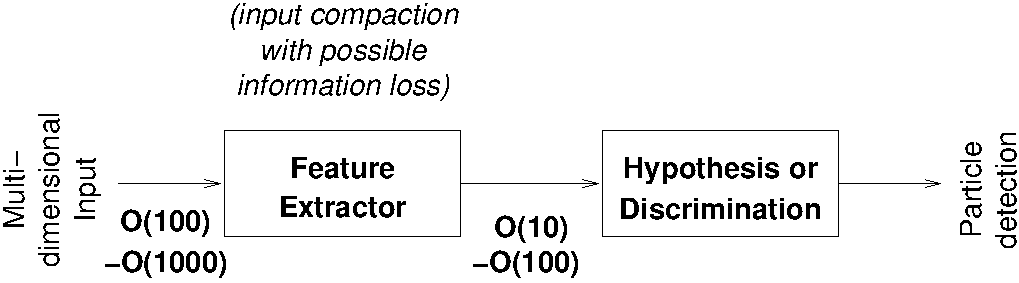
\includegraphics[scale=0.5]{basic-discriminator}
\end{center}
\caption{Um sistema genérico de deteção em um problema de Física de Altas Energias.}
\label{fig:basic-discriminator}
\end{figure}

\begin{enumerate}
\item A \textbf{extração de características}, onde deseja-se compactar a
informação disponível para análise em um mínimo de variáveis que consigam
extrair toda (ou na maior parte) a informação discriminante disponível no
evento. Esta fase é normalmente essencial uma vez que dispõe-se de milhares de
variáveis para cada evento, contando com os elementos de deteção providos pelo
experimento até variáveis complexas que podem ser acessadas após a
reconstrução como o número de jatos encontrados ou o ângulo entre léptons;
\item A \textbf{classificação ou hipótese}, seguindo-se à compressão do espaço
original de entrada representa a deteção da física de interesse. Observa-se
uma tendência ao desenvolvimento dos sistemas utilizando-se dados de simulação
acurados, onde possível, dados provenientes diretamente do detetor. É
interessante perceber que sistemas desenvolvidos através de simulações ainda
comportam-se de forma satisfatória ou adaptativa em seu emprego final, com
dados reais.
\end{enumerate}

Os métodos propostos possuem maior robustez que sua contrapartida e podem ser
executados de forma bastante rápida, em muitas instâncias sendo propostos para
execução em \eng{hardware} especializado. Sistemas especialistas podem ser
empregados em problemas mais complexos, onde deseja-se dedicar cada porção do
detetor a uma atividade bem definida, combinando-se ao final as respostas de
cada sub-sistema para obter um sistema de classificação com uma única saída.

No que se segue deste capítulo, abordaremos sistemas de classificação que
substituem o classificador atualmente empregado na discriminação elétron/jato
para o Segundo Nível do Sistema de Filtragem do experimento ATLAS,
introduzindo técnicas automáticas de deteção. Após definirmos os limites
do processo de compressão estabelecidos pelo extrator de características
T2Calo, tentar-se-á abordar a discriminação elétron/jato através de outras
variáveis que possuam um poder discriminante maior que o sistema proposto
atualmente no CERN.

\subsection{Discriminador de Fisher na separação e\-lé\-tron/jato}
\label{sec:linear}

O discriminador de Fisher \cite{fisher} ou a Análise de Discriminação Linear
descreve um algoritmo para que se maximize a capacidade discriminante de um
corte num plano com N dimensões, que separa duas classes de dados. O resultado
do discriminante é ótimo no caso de dados apresentarem uma distribuição
gaussiana e as matrizes de covariância, para ambas as classes em separado,
serem idênticas\footnote{A Análise de Discriminação Quadrática, no entanto,
demonstra que esta característica pode ser relaxada considerando-se que seja
sempre possível projetar, através de uma transformação linear, o espaço de
entrada em um outro espaço onde as matrizes de covariância sejam iguais e
portanto recaindo no caso simples.}. Em resumo, o discriminante de Fisher
maximiza, através de uma transformação linear, a distância entre as classes
que se deseja detetar, ao mesmo tempo diminuindo a distância de elementos
intra-classe.

Levando-se em consideração as 4 variáveis definidas pelo T2Calo, é possível
encontrar o plano quadri-dimensional que defina um discriminador linear ótimo,
usando-se o algoritmo de retro-propagação resiliente a erros, como descrito
no Apêndice~\ref{ap:rna}. A separação em classes de treinamento e teste, como
apresentada na Seção~\ref{sec:eghypo}, será reaproveitada aqui, para que seja
possível a comparação dos resultados nos dois casos. O fluxo de informação
deste novo sistema está apresentado na
Figura~\ref{fig:t2calo-lms-block}. Nesta nova implementação do algoritmo de
filtragem, substitui-se o discriminador por cortes proposto originalmente, por
um sistema simples de deteção linear.

\begin{figure}
\begin{center}
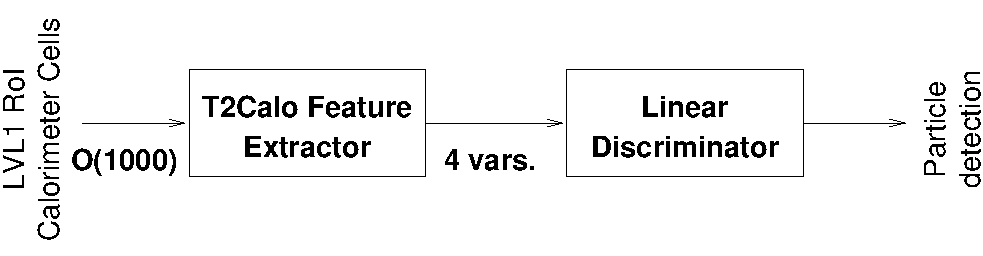
\includegraphics[scale=0.5]{t2calo-lms-block}
\end{center}
\caption{Diagrama de blocos de um sistema de deteção elétron/jato baseado no
Discriminador de Fisher associado ao extrator de características T2Calo.}
\label{fig:t2calo-lms-block}
\end{figure}

O sistema de treinamento e teste foi implementado em um ambiente de trabalho
C++, seguindo o paradigma da orientação a objetos (OO) \cite{stroustrup,
booch}. Este ambiente, que será re-utilizado em várias partes deste trabalho,
é discutido em detalhes no Apêndice~\ref{ap:framework}. A
Figura~\ref{fig:train-flow} contém um diagrama de fluxo com os diversos passos
do sistema de treinamento implementado. Inicialmente, os bancos de dados
usados para o treinamento e teste da rede são carregados. Os valores de média
e variância experimentais, são extraídos do conjunto de treinamento e
guardados juntos aos pesos $\hat{w}(n)$, para que sejam aplicados durante o
treinamento\footnote{De fato, seria mais eficiente que os fatores de
normalização fossem aplicados previamente ao treinamento. No entanto, uma vez
que deseja-se re-aproveitar a base de código para rodar o discriminador em uma
etapa seguinte, é mais simples, do ponto de vista da implementação, que a
normalização seja aplicada como parte do passo de execução do
discriminador.}. Os pesos sinápticos são aleatoriamente inicializados (entre
$-1$ e $+1$). Valores-alvo, para cada uma das classes, são pré-fixados: $-1$
para elétrons e $+1$ para jatos. O processo de treinamento é então
disparado. Para cada época ou batelada\footnote{Os termos \textit{época} e
\textit{batelada} serão usados indistintamente no contexto deste trabalho.}
de treinamento, um conjunto de elétrons e jatos é escolhido aleatoriamente à
partir dos bancos-de-dados disponíveis. Os valores de erro são calculados e
sua média é aplicada para a correção dos pesos sinápticos, considerando a taxa
de aprendizagem $\alpha$. A rede resultante no final do processo de
treinamento é salva e utilizada como o discriminador treinado.

\begin{figure}
\begin{center}
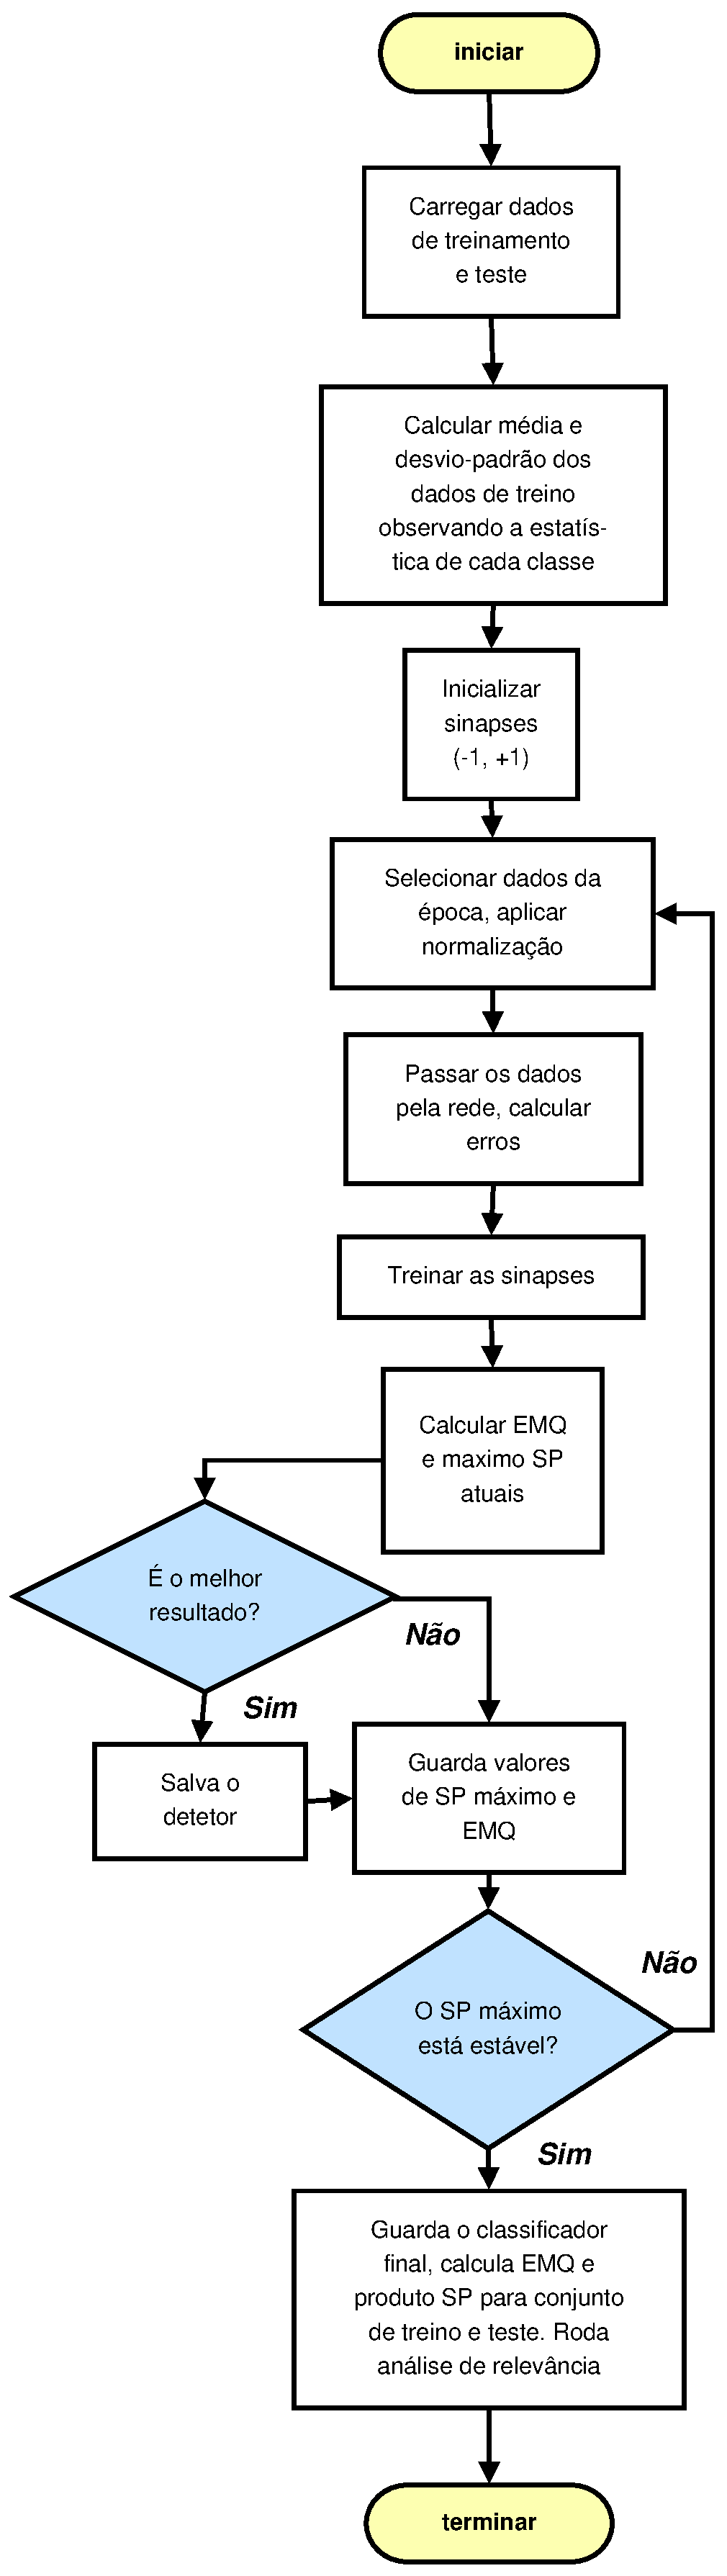
\includegraphics[scale=0.35]{train-flow}
\end{center}
\caption{O fluxo implementado para o treinamento do discriminador linear.}
\label{fig:train-flow}
\end{figure}

Um sistema configurável é utilizado para detetar a estagnação do treinamento e
parar o treinamento do detetor. Para isto, tal sistema baseia-se na observação
do valor do produto SP para o conjunto de teste. Quando este valor atinge um
estado no qual as alterações sinápticas não o modificam significativamente
(levando-se em consideração uma margem de erro configurável e obtida
empiricamente), e por um número de iterações, o treinamento é automaticamente
encerrado. O estado final do discriminador é recarregado. Um estudo dos
valores de Erro Médio Quadrático (\gls{glos:emq}, do inglês \eng{Mean-square
error}, MSE) é feito para os conjuntos de treinamento e teste. O produto SP
máximo também é avaliado para os dois conjuntos de dados. Esta técnica tem o
objetivo de evitar um treinamento excessivo da rede (do inglês
\eng{overtraining}) fazendo com que ela se especialize em demasiado nestes
dados sem atingir uma capacidade de discriminação generalizada. O valor da
variação do produto SP, a partir do qual considera-se que o sistema esteja
estagnado, dependerá do problema. Valores típicos estão na ordem de $10^{-3}$,
para o problema abordado utilizou-se um valor igual a $0,0001$.

Neste trabalho, optou-se pela não utilização de um conjunto de testes distinto
do conjunto de validação. Este conjunto poderia ser utilizado para verificar a
operação do sistema após o treinamento. No entanto, a física disponível para o
estudo é limitada devido a natureza de geração de eventos. Para se realizar
uma análise baseada no LVL2, elétrons e jatos que sejam selecionados por um
corte do LVL1 devem ser simulados, uma vez que o LHC ainda não encontra-se
operacional. Desta forma, os termos \textit{conjunto de teste} e
\textit{conjunto de validação} serão utilizados de forma intercambiável no
contexto deste trabalho.

A taxa de redução do LVL1 é bastante expressiva, atingindo uma supressão de
aproximadamente 1000 vezes na taxa de contaminação de elétrons. Desta forma,
para produzir 1000 jatos que seriam selecionados por um corte do LVL1 é
necessário que se produza cerca de 1 milhão de eventos deste tipo. Cada
simulação de um evento pode durar muitos minutos, às vezes horas de
processamento do poder de computação disponível. Por outro lado, dada a
natureza da geração dos eventos (simulação por processos de Monte Carlo), a
estatística contida no conjunto é tida como suficiente para expressar bem as
características do tipos de evento analisados.

%Por outro lado, a física simulada é representativa do tipo de partículas
%que deseja-se analisar.

\subsection{Resultados para um detetor linear aplicado à separação
e\-lé\-tron-jato}

Utilizando o sistema descrito anteriormente e a separação dos dados (em
classes de treinamento e teste) proposta no início do estudo, realizou-se um
conjunto de 5 testes, com a finalidade de verificar que o mínimo tenha sido
atingido durante o processo de treinamento. Em cada um dos cinco testes os
pesos sinápticos são inicializados aleatoriamente com um valor dentro do
intervalo $[-1, +1]$. O tamanho da época é fixado em 22000 (duas vezes o
número total de elétrons disponíveis para o treinamento), de forma que cada
passo de treinamento represente a informação contida em toda a massa de dados
disponível. 

Dependendo da inicialização, a convergência do sistema (estagnação detetada no
conjunto de teste a partir do produto SP) poderá demorar de 50 a 70 passos
para ser estabelecida pelo programa. O valor do EMQ na saída do detetor
treinado é ligeiramente diferente para os 5 casos, variando entre $0,3818$ e
$0,3825$. O valor do produto SP no final do treinamento está entre $1,477$ e
$1,479$, também dependendo do ponto de parada.

A Figura~\ref{fig:lms-mse-evo} mostra a evolução do EMQ para a melhor das 5
redes, tanto para o conjunto de treinamento quanto para o conjunto de teste. A
Figura~\ref{fig:lms-sp-evo} mostra um gráfico equivalente, mas para o produto
SP, ao invés do EMQ. Como é possível verificar pelo valor desta variável, o
sistema converge a um valor estável depois de pouco menos que 20 passos de
treinamento. O produto SP oscila bruscamente no início do treinamento, por
cerca de 10 passos, e depois se estabiliza, em aproximadamente $1,48$, para o
restante do treinamento. O mesmo ocorre para o EMQ para um valor de
aproximadamente $0,38$. O perfil de evolução do produto SP e a minimização do
EMQ é seguido pelo conjunto de teste, de forma bastante semelhante, indicando
que a estatística disponível no conjunto treino é representativa dos dados
no conjunto de teste.

%É interessante notar que após 20 passos de treinamento, $10000$
%elementos terão sido utilizados no treinamento da rede. Este valor é menor que
%o tamanho do conjunto de treinamento, com cerca de $15000$ elementos,
%indicando que o conjunto de dados, para a análise linear, ...

\begin{figure}
\begin{center}
\includegraphics[scale=0.98]{lms/mse-evolution}
\end{center}
\caption{Evolução dos valores do EMQ ao longo do treinamento do detetor
linear, para o conjunto de treinamento e de teste.}
\label{fig:lms-mse-evo}
\end{figure}

\begin{figure}
\begin{center}
\includegraphics[scale=0.98]{lms/sp-evolution}
\end{center}
\caption{Evolução dos valores do produto SP ao longo do treinamento do detetor
linear, para o conjunto de treinamento e de teste.}
\label{fig:lms-sp-evo}
\end{figure}

A Figura~\ref{fig:lms-test-output} mostra os histogramas da saída da rede para
elétrons e jatos, considerando-se o conjunto de teste. O ponto ótimo de corte,
determinado para que se maximize o produto SP da rede para o conjunto de
treinamento para este sistema é $-0,436$. No caso em questão, observa-se que,
possivelmente, os conjuntos de dados não sejam linearmente separáveis, dado
que a saída do detetor, tanto para elétrons quanto para jatos, se superpõe em
parte do espectro de saída do sistema. Nestas condições, o máximo produto SP
para o conjunto de teste é 1,48, definido no ponto da curva R.O.C. (veja
Figura~\ref{fig:lms-test-roc}) onde a eficiência para a deteção de elétrons é
90,77\%, enquanto que a eficiência para a deteção de jatos é de 90,21\%. A
Figura~\ref{fig:lms-vs-egamma-roc} mostra uma comparação entre o resultado da
otimização proposto atualmente no experimento ATLAS contra os resultados
obtidos para este classificador. Através desta figura é possível observar que
o discriminador linear praticamente tangencia a parte exterior dos pontos da
otimização proposta atualmente no experimento. O resultado obtido com este
sistema de discriminação, ao invés do longo processo de otimização proposto
originalmente, é atingido depois de apenas alguns minutos de treinamento em um
computador dotado de um processador AMD 64 com \eng{clock} de 2~GHz e 1~Gb de
memória RAM. Ademais, tal sistema apresenta uma capacidade discriminatória
equivalente após apenas 10 passos de treinamentos, isto é, $\approx 25$
segundos na máquina citada. Esta nova ferramenta oferece algo que o EGammaHypo
jamais poderá: a atualização dos pesos sinápticos poderá ser feita rapidamente
para se arcar com a mudança de condições no experimento.

\begin{figure}
\begin{center}
\includegraphics[scale=0.98]{lms/test-output}
\end{center}
\caption{Saída do discriminador linear (após treinamento) para elétrons e
jatos.}
\label{fig:lms-test-output}
\end{figure}

\begin{figure}
\begin{center}
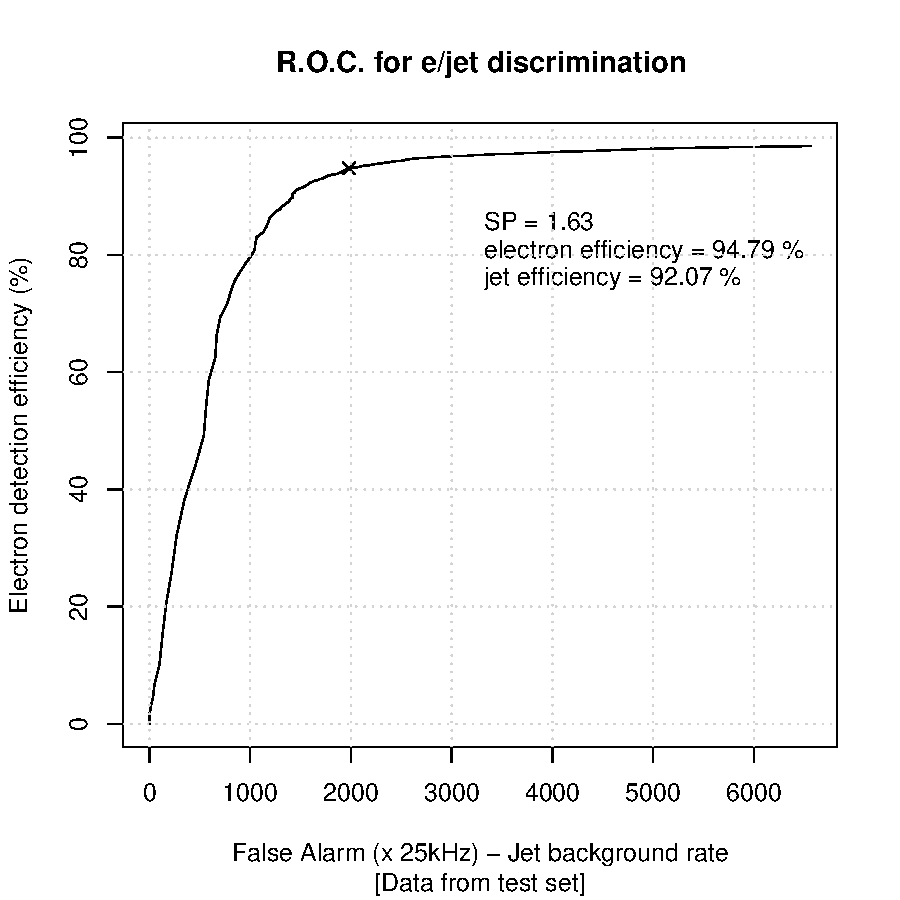
\includegraphics[scale=0.98]{lms/test-roc}
\end{center}
\caption{Curva R.O.C. para um detetor linear para elétrons e jatos baseado nas
4 variáveis do T2Calo, usadas para discriminação pelo EGammaHypo.}
\label{fig:lms-test-roc}
\end{figure}

\begin{figure}
\begin{center}
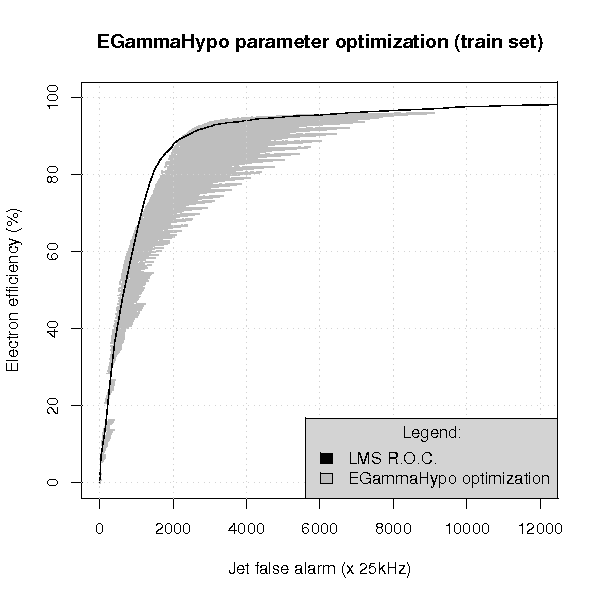
\includegraphics[scale=0.98]{lms/lms-vs-egamma-roc}
\end{center}
\caption{R.O.Cs comparativas entre a otimização atual para o EGammaHypo e um
detetor linear.}
\label{fig:lms-vs-egamma-roc}
\end{figure}

As Figuras~\ref{fig:lms-test-eta-phi} e \ref{fig:lms-test-efficiency-et}
mostram, respectivamente, o valor do produto SP segundo a distribuição dos
dados em $\eta\times\phi$ e $\etem$. O número anexo ao topo de cada barra
(gráficos do produto SP) indica a quantidade, separadamente, de elétrons e
jatos em cada canal e é útil para que se considere a importância de um valor
parcial no desempenho do discriminador. Nota-se que na distribuição por
$\eta$, há uma clara perda de eficiência na região $|\eta| \approx 1,5$. Esta
notável queda no desempenho do classificador é devido a um espaço sem
elementos de deteção nesta área (também conhecido como \eng{gap} ou
\eng{crack} dos calorímetros), por onde passam os cabos de leitura e
manutenção dos detetores internos. Como mostra a
Figura~\ref{fig:lms-test-eta-phi}(a), a perda devido à esta região do sistema
sem elementos de deteção, está diretamente relacionada à eficiência de deteção
de elétrons. Isto acontece pois elétrons desenvolvem uma cascata de deposição
energética tipicamente mais fina e de pouca penetração, estando,
adicionalmente, sujeitos à interação com os cabos do detetor. Jatos, por sua
vez, tenderão a penetrar mais no detetor e se radializar, o que facilita a
recuperação da informação mesmo em regiões mais difíceis, como o
\eng{crack}.

\begin{figure}
\begin{center}
\mbox{%
 \subfigure[Eficiência por $\eta$]{\includegraphics[scale=0.49]{lms/test-efficiency-eta}}%
 \subfigure[Eficiência por $\phi$]{\includegraphics[scale=0.49]{lms/test-efficiency-phi}}%
}
\mbox{%
 \subfigure[Produto SP por $\eta$]{\includegraphics[scale=0.49]{lms/test-sp-eta}}%
 \subfigure[Produto SP por $\phi$]{\includegraphics[scale=0.49]{lms/test-sp-phi}}%
}
\end{center}
\caption{Análise da eficiência de classificação e do produto SP para o
classificador linear, para os dados do conjunto de teste ao longo de $\eta$ em
(a) e (c) e por $\phi$, em (b) e (d).}
\label{fig:lms-test-eta-phi}
\end{figure}

\begin{figure}
\begin{center}
\subfigure[Eficiência]{\includegraphics[scale=0.6]{lms/test-efficiency-emet}}
\subfigure[Produto SP]{\includegraphics[scale=0.6]{lms/test-sp-emet}}
\end{center}
\caption{Análise da eficiência de deteção de elétrons e falso-alarme em jatos
(a) e do produto SP (b) por $\etem$ para o classificador linear, tendo por
base os dados do conjunto de teste.}
\label{fig:lms-test-efficiency-et}
\end{figure}

% Old arrangements w/o subfigure usage
%\begin{figure}
%\begin{center}
%\includegraphics[scale=0.98]{lms/test-sp-emet}
%\end{center}
%\caption{Análise do produto SP do classificador linear, para os dados do
%conjunto de teste por $\etem$.} 
%\label{fig:lms-test-sp-emet}
%\end{figure}

%\begin{figure}
%\begin{center}
%\includegraphics[scale=0.98]{lms/test-efficiency-eta}
%\end{center}
%\caption{Análise da eficiência de deteção de elétrons e falso-alarme em jatos
%por $\etem$ para o classificador linear, tendo por base os dados do conjunto
%de teste.}
%\label{fig:lms-test-efficiency-eta}
%\end{figure}

A eficiência é recuperada logo após a região do \eng{crack}. O gráfico de
barras para a distribuição $\phi$ mostra-se praticamente uniforme, indicando
que o sistema funciona sem tendências para todos os valores desta
variável. Este resultado é esperado, já que o detetor é simétrico neste
eixo. A análise por $\etem$ demonstra uma predominante qualidade de deteção
para valores mais baixos de energia do que para valores mais altos. Deve-se
levar em conta que, embora a eficiência de deteção de elétrons ainda seja
máxima nesta última região, como mostra a
Figura~\ref{fig:lms-test-efficiency-et}(a), o falso alarme na deteção de jatos
também apresenta-se máximo. Uma vez que o produto SP é uma figura de mérito da
eficiência agregada de ambas as classes de eventos do discriminador, ela
quantificar-se-á em zero nesta região. Este resultado está, possivelmente,
associado à baixa estatística de dados disponível na região, como indicado no
texto sob as barras. Desta forma, a análise de valores de eficiência de
deteção para objetos com mais de $~$50 GeV deverá ser tomada com esta
ressalva.

A Figura~\ref{fig:lms-vs-egamma} mostra uma comparação entre as duas técnicas
de deteção, por energia transversa na seção e.m.. Por inspeção desta figura,
distingue-se que os dois sistemas possuem respostas bastante próximas. Na
primeira (mais à esquerda) faixa de energia considerada, o EGammaHypo possui
uma resposta melhor, enquanto que com o aumento da energia transversa o detetor
linear apresenta-se mais eficiente, e segue este padrão para grande parte das
faixas onde se diferenciam (15 pontos no total). Na região onde há maior
concentração de eventos de teste, como é possível determinar a partir da
Figura~\ref{fig:lms-test-efficiency-et}, o desempenho dos detetores é muito
próximo. Com o aumento da energia, onde a eficiência do EGammaHypo começa a
cair, o sistema baseado no detetor linear consegue obter bom desempenho
superando o primeiro.

\begin{figure}
\begin{center}
\includegraphics[scale=0.98]{lms/et-compare}
\end{center}
\caption{Comparação do produto SP para o classificador linear e o
EGammaHypo por energia transversa na seção e.m..}
\label{fig:lms-vs-egamma}
\end{figure}

Levando-se em consideração a saída do detetor, na
Figura~\ref{fig:lms-test-output}, compreende-se que este método de deteção não
apresente a robustez necessária ao experimento. Conclui-se, a partir desta
saída, que os objetos das duas classes de dados não sejam linearmente
separáveis.

\section{Métodos neurais de discriminação}
\label{sec:neural}

Redes neurais artificiais (RNA) vêm sendo atualmente utilizadas com sucesso em
problemas de otimização, controle e reconhecimento de padrões
\cite{haykin}. RNA's são modelos matemáticos inspirados no conhecimento
limitado que temos do cérebro animal. Neste contexto, entende-se que uma rede
neural pode aprender através do contato com os elementos de interesse de um
determinado espaço de entrada e que este conhecimento é armazenado através das
conexões sinápticas que conectam os elementos processadores (neurônios) da
rede. Dentre as características interessantes destacam-se para o problema
atual:

\begin{description}
\item[Robustez] Sistemas neurais, por tentarem recortar o espaço de variáveis
de entrada de forma mais sofisticada que sistemas lineares, normalmente
atingem um nível de separação entre as classes de objetos superior a outros
detetores. Esta qualidade é fundamental em ambientes onde a informação de
entrada no sistema de deteção nem sempre está completa. Especificamente no
experimento ATLAS, dada a grande complexidade do sistema, é possível que
determinadas regiões do detetor sejam omitidas pelo sistema de leitura devido
a panes de naturezas diversas. Neste contexto, contar com um sistema que ainda
conseguirá obter um bom nível de discriminação apesar destas condições
torna-se muito vantajoso;

\item[Generalização] RNA's podem extrair a informação relevante escondida sob
uma grande quantidade de ruído e portanto poderão detetar canais físicos não
simuláveis no caso de exibirem propriedades equivalente àquelas para o qual
foram treinadas. Num ambiente de descobertas, como é o experimento ATLAS, esta
característica torna-se fundamental uma vez que a Física de interesse pode se
apresentar num formato pouco evidente a sistemas clássicos de deteção;

\item[Simples implementação] RNA's podem ser facilmente descritas em
linguagens de programação convencionais, atingindo desempenhos satisfatórios
para um grande conjunto de aplicações em tempo real. Esta característica torna
RNA's atrativas para implementação em ambientes como o Sistema de Filtragem do
experimento ATLAS, onde os tempos de processamento e a utilização de recursos
são bastante reduzidos.
\end{description}

RNA's podem ser implementadas de várias maneiras, incluindo sistemas com
percéptrons com apenas uma ou múltiplas camadas (do inglês, \eng{multi-layer
perceptron}, ou \gls{glos:mlp}), incluindo sistemas realimentados ou híbridos
\cite{haykin}. O processo de aprendizagem ou aproximação da resposta à saída
desejada no sistema é conduzido normalmente por uma fase de treinamento, que
poderá ser realizado, igualmente, de maneiras distintas. Duas grandes
sub-categorias são reconhecíveis: métodos supervisionados e
não-supervisionados.

Na aprendizagem supervisionada, o desenvolvedor utiliza-se de uma informação
de conhecimento \textit{a priori} da função que deseja executar para reprimir
ou reforçar a migração do sistema na direção adequada. Uma das grandes
dificuldades neste tipo de aprendizagem é a definição de um algoritmo de
treinamento que convirja de forma adequada ao problema que se deseja atender.

Muito algoritmos foram desenvolvidos para as diversas estruturas de rede,
dentre os quais, a retropropagação de erros tornou-se um dos mais populares em
aplicações ligadas a Física de Altas Energias. No treinamento por
retropropagação de erros, os sinais de erro são propagados a partir da saída
da rede, onde são medidos, para os neurônios escondidos através de um
mecanismo análogo ao algoritmo LMS, para o treinamento do sistema linear
estudado anteriormente. A retropropagação de erros aplicada a redes neurais
artificiais é revista com mais detalhes no Apêndice~\ref{ap:rna}. Este método
possui, no entanto, muitos problemas para a determinação dos parâmetros ótimos
de treinamento. Como variação dos métodos explorados normalmente em Física de
Altas Energias, e no intuito de buscar-se um método mais robusto e livre de
parâmetros de treinamento, utilizaremos uma variante do treinamento por
retropropagação de erros conhecida como \textit{retropropagação de erros
resiliente} (do inglês \eng{resilient backpropagation}, \gls{glos:rprop})
\cite{rprop}. Esta técnica também encontra-se descrita no apêndice.

Em específico, o problema da separação elétron/jato como se apresenta ao
detetor EGammaHypo e ao sistema de deteção linear (treinado pelo LMS), indica
que correlações não lineares estejam presentes no sistema. De fato, a
inseparabilidade linear através das variáveis do T2Calo pode ser facilmente
inspecionada através das distribuições das duas variáveis mais discriminantes
deste extrator de características, na Figura~\ref{fig:eratio-vs-rcore}.

\begin{figure}
\begin{center}
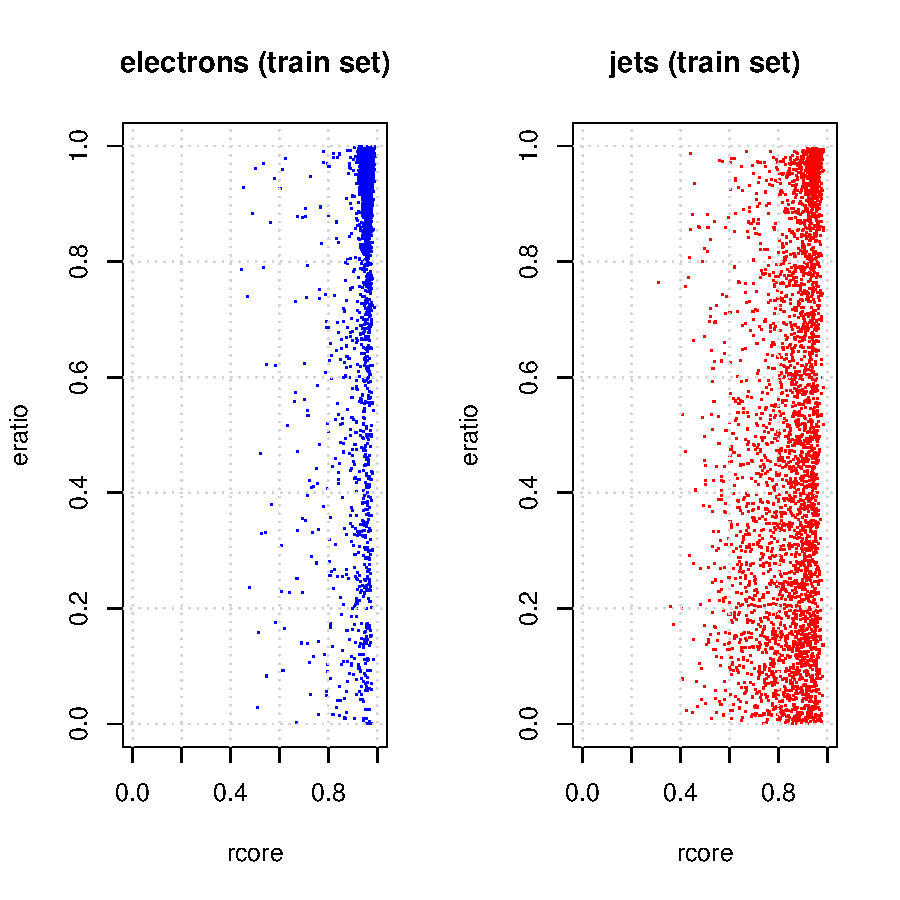
\includegraphics[scale=0.6]{eratio-vs-rcore.pdf}
\end{center}
\caption{Gráfico de dispersão mostrando a distribuição das duas variáveis mais
discriminantes para o T2Calo, para as classes de elétrons e jatos.}
\label{fig:eratio-vs-rcore}
\end{figure}

Não obstante, a qualidade da discriminação é comparável ao sistema de deteção
proposto pelo algoritmo EGammaHypo, não necessitando da intervenção de um
especialista para seu ajuste. Se por um lado são compatíveis, estes dois
sistemas de deteção mostram-se pouco robustos a mudanças de condição como as
que serão observadas no experimento ATLAS, onde a luminosidade do feixe está
sujeita a bruscas variações em questão de minutos. Na seção que se segue,
analisa-se o potencial discriminatório que redes neurais artificiais
adicionariam ao sistema de filtragem do ATLAS.

Para o treinamento e implementação dos sistemas de discriminação neural,
fez-se uso das bibliotecas e programas do \eng{NeuralRinger}. O
\eng{NeuralRinger} é um pacote totalmente desenvolvido usando o paradigma da
orientação a objetos, implementado em C++ \cite{stroustrup, booch} e
especialmente concebido para executar a operação de filtragem de partículas
dentro do LVL2. Outras soluções para treinamento e execução de redes neurais,
tais como o pacote SNNS \cite{snns} foram investigadas antes do
desenvolvimento deste sistema. Entretanto, os pacotes em questão são
normalmente utilizados para uma grande variedade de sistemas neurais. Esta
flexibilização muito freqüentemente ocorre em detrimento do desempenho em
casos específicos. Ademais, ao usar um sistema tão genérico, estaria-se
inserindo uma grande quantidade de código dentro do sistema de filtragem, que
seria, em sua maior parte, pouco ou não utilizada.

As escolhas do paradigma de programação e da linguagem de implementação C++
ocorreram em função do ambiente-alvo para este sistema. Como colocado na
Seção~\ref{sec:hlt}, o LVL2 de filtragem rodará utilizando como base as
bibliotecas do Projeto Athena. O Athena é o ambiente padrão para a análise da
Física dos eventos no ATLAS, tanto no Sistema de Filtragem, como na
Reconstrução pós-filtragem nas diversas \eng{farms} de análise
\eng{offline}. Desta forma, a integrabilidade ao Athena constitui-se um
passo essencial para a utilização da técnica no LVL2.

O projeto foi desenvolvido tendo por base as seguintes prerrogativas, em
ordem:

\begin{enumerate}
\item Otimização da execução de redes neurais: É importante que o sistema
tenha um bom desempenho no processamento neural, de tal forma que seja viável
sua implementação no sistema de filtragem. Preferencialmente, deseja-se que um
passo de execução da rede não dure mais que alguns milissegundos, já que o
tempo total de processamento no LVL2 deve ser em média 10~ms, contando com o
acesso aos dados;
\item Interoperabilidade: O treinamento do sistema deve ser executado
\eng{offline}, dada a disponibilidade dos dados. Portanto, é necessário que o
sistema opere tanto dentro do ambiente Athena, quanto em modo desacoplado;
\item Multi-tarefas: Respeitando o projeto do LVL2, o \eng{NeuralRinger} não
deve ter construções que impossibilitem ou dificultem a sua utilização
concorrente em múltiplas tarefas;
\item Configurabilidade: O \eng{NeuralRinger} deve ser, dentro de determinadas
medidas, configurável e flexível com relação à configuração da rede que será
usada na deteção dos alvos. O método de treinamento a ser utilizado será a
retro-propagação de erros resiliente, tendo por base redes totalmente
conectadas e sem re-alimentação.
\end{enumerate}

O Apêndice~\ref{ap:framework} traz detalhes do projeto e implementação
desta ferramenta.

\subsection{Discriminação neural aplicada às saídas do T2Calo}

É possível substituir o discriminador linear definido na
Seção~\ref{sec:linear} por um discriminador baseado em uma rede neural tipo
MLP como a da Figura~\ref{fig:simple-mlp}. A implementação deste novo sistema
utilizando-se do pacote \eng{NeuralRinger} segue o fluxo de treinamento foi
detalhado na Figura~\ref{fig:train-flow}. A Figura~\ref{fig:t2calo-neural}
contém um diagrama de blocos que ilustra tal sistema. Os conjuntos de
treinamento e teste serão mantidos, o que simplificará a comparação das duas
técnicas.

\begin{figure}
\begin{center}
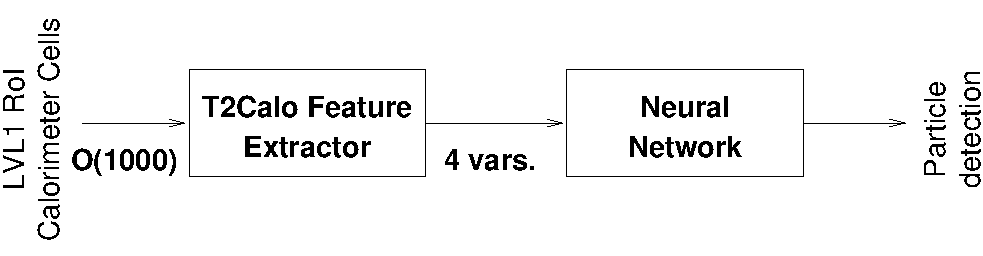
\includegraphics[scale=0.9]{t2calo-neural}
\end{center}
\caption{Um discriminador neural para as características definidas pelo
T2Calo.}
\label{fig:t2calo-neural}
\end{figure}

Uma vez que estamos utilizando o algoritmo de retropropagação de erros
resiliente, o único parâmetro a ser otimizado é o número de neurônios
escondidos. Para procedermos com a escolha, a seguinte heurística será
utilizada: realizam-se 5 testes com um número fixo de neurônios na camada
escondida. Em seguida, avalia-se o número de passos de treinamento para um
nível de estabilização fixo do produto SP, o valor final do EMQ e do produto
SP da rede. A média dos cinco valores é extraída, assim como o desvio padrão
destes valores em relação à média. O número de neurônios escondidos a ser
considerado está no conjunto $[2, 3, 4, 5, 6]$. A
Tabela~\ref{tab:t2calo-neural-hidden-scan} contém os resultados deste
estudo. O valor do desvio padrão está anotado após o sinal ``$\pm$'' em cada
entrada da tabela. Como é possível observar, com 4 neurônios escondidos o
sistema tende a ser treinado em um número menor de passos. Os valores de EMQ e
o produto SP encontram-se em faixas de valores muito próximas, sendo difícil
sua comparação para fins de escolha. Desta forma, escolhe-se o sistema com 4
neurônios na camada escondida.

\begin{table}
\caption{Resultados da otimização do número de neurônios escondidos para um
discriminador neural elétron/jato baseado na saída do T2Calo.}
\label{tab:t2calo-neural-hidden-scan}
\begin{center}
\begin{tabular}{|r|r|r|r|r|r|} \hline
N & Passos & EMQ/teste & EMQ/treino & SP/teste & SP/treino \\
\hline 
%$1$ & $176\pm63$ & $0,264\pm0,001$ & $0,255\pm0,001$ & $1,546\pm0,002$ & $1,543\pm0,001$ \\
$2$ & $232\pm54$ & $0,261\pm0,002$ & $0,252\pm0,003$ & $1,543\pm0,004$ & $1,542\pm0,003$ \\
$3$ & $232\pm66$ & $0,262\pm0,002$ & $0,253\pm0,002$ & $1,543\pm0,002$ & $1,543\pm0,001$ \\
$4$ & $154\pm42$ & $0,261\pm0,003$ & $0,253\pm0,003$ & $1,541\pm0,002$ & $1,541\pm0,002$ \\
$5$ & $206\pm130$ & $0,263\pm0,003$ & $0,254\pm0,003$ & $1,545\pm0,001$ & $1,545\pm0,003$ \\
$6$ & $332\pm138$ & $0,258\pm0,004$ & $0,249\pm0,004$ & $1,545\pm0,001$ & $1,546\pm0,003$ \\
\hline
\end{tabular}
\end{center}
\end{table}

Em seguida, treina-se um total de 10 redes com os parâmetros
selecionados. Para nos assegurarmos da estabilidade da rede, estabelece-se
como critério de parada, uma variação menor que $0,0001$ para o produto SP,
por pelo menos 20 passos de treinamento. As
Figuras~\ref{fig:best-t2calo-mlp-mse} e \ref{fig:best-t2calo-mlp-sp} mostram,
respectivamente, o desenvolvimento ao longo do treinamento, dos valores EMQ e
do produto SP para um dos 10 resultados obtidos.

\begin{figure}
\begin{center}
\includegraphics[scale=0.6]{t2calo-mlp/mse-evolution}
\end{center}
\caption{Evolução do EMQ para os conjuntos de treino e teste de um
discriminador elétron/jato neural para as variáveis do T2Calo.}
\label{fig:best-t2calo-mlp-mse}
\end{figure}

\begin{figure}
\begin{center}
\includegraphics[scale=0.6]{t2calo-mlp/sp-evolution}
\end{center}
\caption{Evolução do produto SP para os conjuntos de treino e teste de um
discriminador elétron/jato neural para as variáveis do T2Calo.}
\label{fig:best-t2calo-mlp-sp}
\end{figure}

O sistema estabiliza após cerca de 40 passos, considerando a evolução do
EMQ. No que tange à capacidade discriminante, aferida através do produto SP,
após cerca de 60 passos, a qualidade discriminativa parece estar estável. A
Figura~\ref{fig:best-t2calo-mlp-output} mostra as saídas da rede, no final do
treinamento, para elétrons (em cima) e jatos (em baixo). A saída para elétrons
é fixada em $-1$ e para jatos, em $+1$. Nota-se que, diferente do sistema
linear, há uma notável separação entre as classes, proporcionada pelo emprego
de um discriminador neural. O ponto ótimo de separação pode ser mais
facilmente determinado, inclusive por inspeção visual, o que torna este sistema
mais robusto que os propostos anteriormente.

\begin{figure}
\begin{center}
\includegraphics[scale=0.98]{t2calo-mlp/test-output}
\end{center}
\caption{Saída para o conjunto de teste, do discriminador neural baseado nas
características extraídas pelo T2Calo.}
\label{fig:best-t2calo-mlp-output}
\end{figure}

Diferentemente do sistema linear, uma rede neural poderá traçar uma superfície
curva no espaço de entrada (número de dimensões $=4$), melhorando a separação
entre as classes que se deseja detetar. A
Figura~\ref{fig:best-t2calo-mlp-output} mostra o resultado desta capacidade
discriminativa. Na Figura~\ref{fig:best-t2calo-test-roc} vemos uma comparação
entre as técnicas de deteção vistas até aqui. Nota-se que o detetor baseado em
uma rede neural com 4 neurônios escondidos exibe superior poder de deteção
comparando-se às outras duas técnicas. A curva para este detetor está sempre
acima da curva dos outros sistemas, indicando superior eficiência de deteção e
rejeição de falso alarme.

\begin{figure}
\begin{center}
\includegraphics[scale=0.98]{t2calo-mlp/roc-compare}
\end{center}
\caption{R.O.C. para o conjunto de teste, do discriminador neural baseado nas
características extraídas pelo T2Calo, comparado com o detetor linear e a
técnica de otimização baseado no algoritmo EGammaHypo.}
\label{fig:best-t2calo-test-roc}
\end{figure}

O valor do produto SP máximo na curva para o detetor neural está nas
coordenadas onde a deteção de elétrons é igual a $92,38\%$ e o falso-alarme em
jatos é apenas $9,05\%$ ($\approx 2,20$~kHz de falso-alarme). Estes valores
correspondem a um produto SP de $1,54$, tal qual ao caso do discriminador
LMS. Uma verificação das eficiências parciais por região em $\eta$ e em $\phi$
revelam uma estrutura bastante semelhante aos sistemas de deteção precedentes,
como mostra a Figura~\ref{fig:best-t2calo-eta-phi}. A única ressalva é a na
qualidade de deteção no \eng{crack} dos calorímetros, onde o detetor neural
mostra-se ligeiramente superior, indicando que este sistema consiga recuperar
informações vitais à deteção que os outros dois métodos não conseguem.

\begin{figure}
\begin{center}
\mbox{%
 \subfigure[Eficiência por $\eta$]{\includegraphics[scale=0.49]{t2calo-mlp/test-efficiency-eta}}%
 \subfigure[Eficiência por $\phi$]{\includegraphics[scale=0.49]{t2calo-mlp/test-efficiency-phi}}%
}
\mbox{%
 \subfigure[Produto SP por $\eta$]{\includegraphics[scale=0.49]{t2calo-mlp/test-sp-eta}}%
 \subfigure[Produto SP por $\phi$]{\includegraphics[scale=0.49]{t2calo-mlp/test-sp-phi}}%
}
\end{center}
\caption{Análise da eficiência de classificação e do produto SP para o
discriminador neural baseado nas saídas do T2Calo, para os dados do conjunto
de teste ao longo de $\eta$ em (a) e (c) e por $\phi$, em (b) e (d).}
\label{fig:best-t2calo-eta-phi}
\end{figure}

%\begin{figure}
%\begin{center}
%\includegraphics[scale=0.98]{t2calo-mlp/test-sp-eta}
%\end{center}
%\caption{Análise do produto SP ao longo de $\eta$ para o discriminador neural
%baseado nas saídas do T2Calo.}
%\label{fig:best-t2calo-test-sp-eta}
%\end{figure}

%\begin{figure}
%\begin{center}
%\includegraphics[scale=0.98]{t2calo-mlp/test-sp-phi}
%\end{center}
%\caption{Análise do produto SP ao longo de $\phi$ para o discriminador neural
%baseado nas saídas do T2Calo.}
%\label{fig:best-t2calo-test-sp-phi}
%\end{figure}

A Figura~\ref{fig:best-t2calo-test-efficiency-et} mostra o valor relativo do
produto SP por faixa de energia transversa na seção e.m.. Uma comparação entre
os 3 métodos do produto SP por faixas de energia descritos até agora se segue
na Figura~\ref{fig:best-t2calo-versus-others-emet}. Os dados nesta figura
correspondem aos do conjunto de teste, para um corte efetuado em $-0,243$ para
o discriminador neural, e para os melhores resultados obtidos com os outros
dois sistemas de deteção de forma equivalente.

\begin{figure}
\begin{center}
\subfigure[Eficiência]{\includegraphics[scale=0.6]{t2calo-mlp/test-efficiency-emet}}
\subfigure[Produto SP]{\includegraphics[scale=0.6]{t2calo-mlp/test-sp-emet}}
\end{center}
\caption{Análise da eficiência de deteção de elétrons e falso-alarme em jatos
(a) e do produto SP (b) por $\etem$ para o discriminador neural baseado nas
saídas do T2Calo, tendo por base os dados do conjunto de teste.}
\label{fig:best-t2calo-test-efficiency-et}
\end{figure}

\begin{figure}
\begin{center}
\includegraphics[scale=0.98]{t2calo-mlp/et-compare}
\end{center}
\caption{Comparação do produto SP para os 3 detetores abordados até aqui, por
faixa de energia e.m. transversa.}
\label{fig:best-t2calo-versus-others-emet}
\end{figure}

É possível notar que o sistema neural ganha em praticamente todas as faixas
energéticas, sobretudo onde existe maior concentração de eventos ($e_T<50
GeV$). No final do espectro observa-se que o detetor neural possui eficiência
de deteção igual a 100\% para ambas as classes de partículas. Como colocado
anteriormente, este resultado é questionável, em virtude da carência de dados
nesta região. A Figura~\ref{fig:t2calo-mlp-best-net} mostra o estado final da
rede neural, após o treinamento, a título ilustrativo.

\begin{figure}
\begin{center}
\begin{sideways}
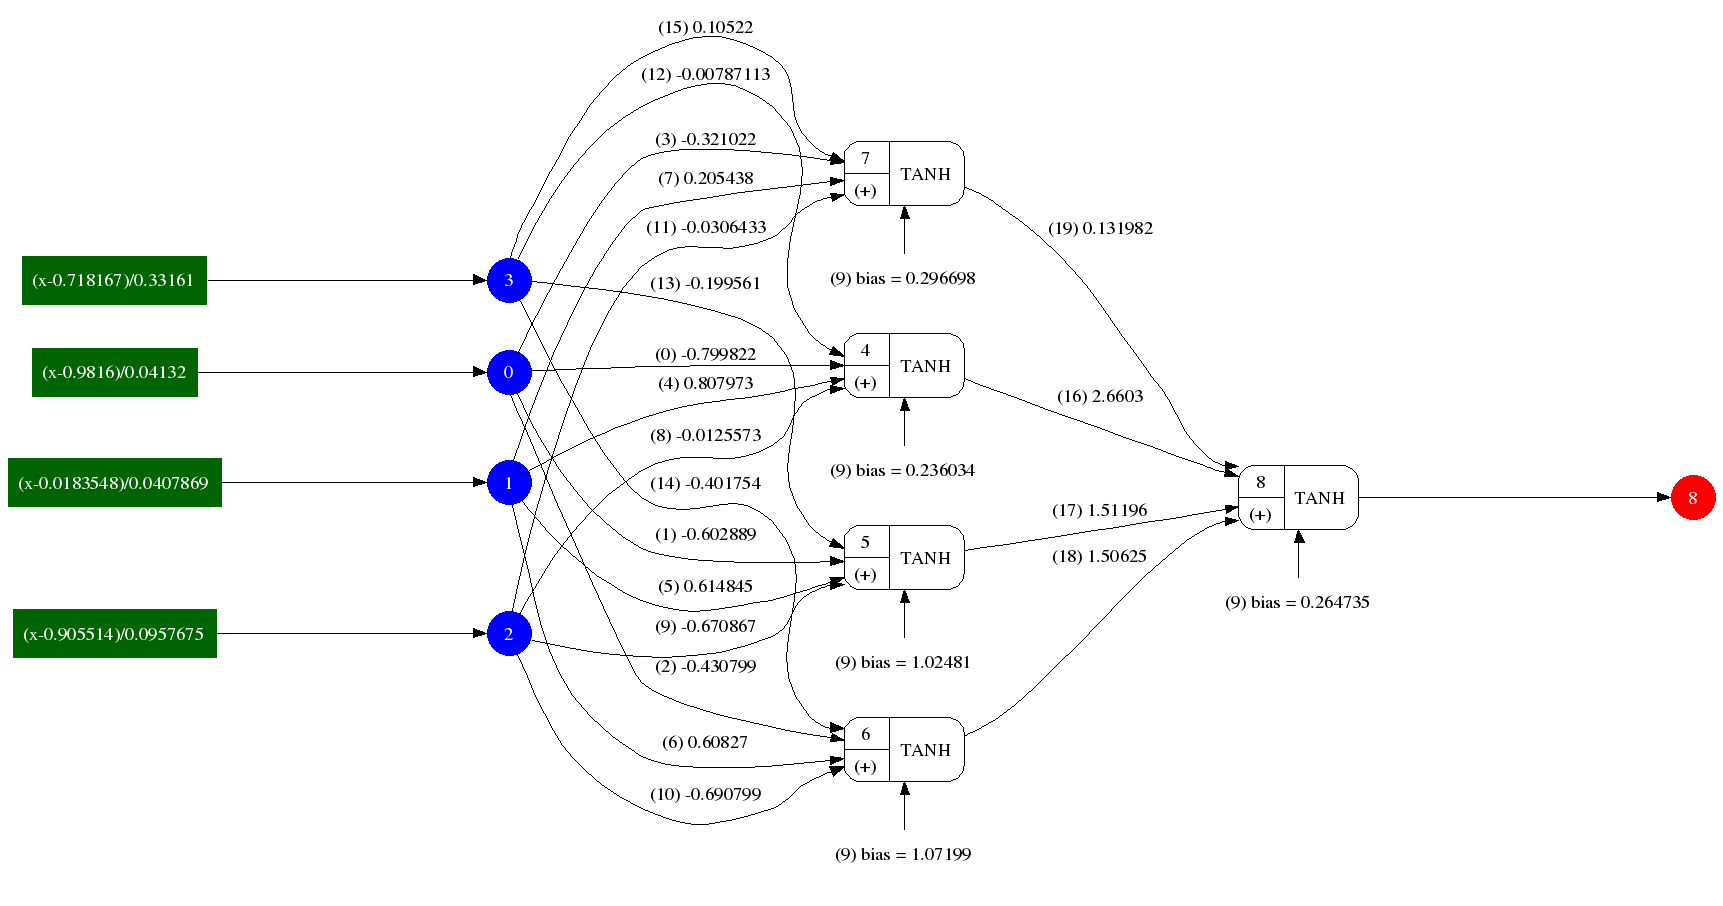
\includegraphics[scale=0.30]{t2calo-mlp/mlp-end}
\end{sideways}
\end{center}
\caption{Diagrama de fluxo do sistema de deteção elétron/jato, neural, usando as
características do T2Calo como entrada.}
\label{fig:t2calo-mlp-best-net}
\end{figure}

\subsection{Adicionando mais variáveis}

Na utilização de discriminação baseada em redes neurais para a Física de Altas
Energias, observa-se uma tendência à re-análise das características utilizadas
pelo sistema de deteção. Isto se deve a capacidade que redes neurais possuem
em extrair correlações de ordem elevada entre as entradas de um detetor,
atingindo desempenhos de discriminação superiores a sistemas baseados em
cortes uni ou bi-dimensionais. Nestes casos, o especialista deve tomar cuidado
em não povoar seu espaço de discriminação com muitas variáveis, o que
tornaria o processo de decisão demasiado complicado. Uma vez que propõe-se o
uso de redes neurais como sistema de discriminação, é possível, até certo
ponto, ignorar esta limitação.

Como sub-produto do cálculo das 4 variáveis utilizadas pelo EGammaHypo, o
T2Calo também avalia, dentre outras, a energia, camada a camada do
calorímetro, depositada pela partícula na RoI sendo analisada. Estas
variáveis, normalmente desprezadas para fins de filtragem, podem conter
informação não originalmente aproveitada pelo EGammaHypo, mas que revele
novos detalhes sobre a natureza da partícula. No total 10 outras variáveis
estão disponíveis:

\begin{itemize}
\item Energias parciais nas 4 camadas da seção e.m. dos calorímetros;
\item Energias parciais nas 4 camadas da seção hadrônica dos calorímetros;
\item A largura do objeto, medida em função da distribuição energética na
segunda camada e.m. dos calorímetros;
\item A relação de deposição energética entre uma região de $3\times7$ células
na direção $\eta\times\phi$ e uma região de $7\times7$ células na segunda
camada e.m..
\end{itemize}

Estas variáveis são usadas normalmente \eng{offline} para a depuração do
comportamento do T2Calo durante sua execução no sistema de filtragem. Enquanto
combinar estas variáveis no algoritmo EGammaHypo seria difícil, o sistema de
discriminação neural proposto na seção anterior poderia ser re-utilizado para
montar-se um novo sistema de deteção baseado em um universo de variáveis maior
e com mais informações. A Figura~\ref{fig:t2calo-14-neural} ilustra este novo
sistema, em blocos.

\begin{figure}
\begin{center}
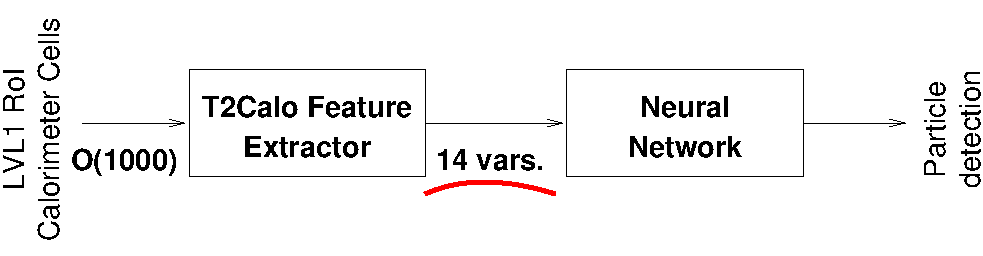
\includegraphics[scale=0.8]{t2calo-14-neural}
\end{center}
\caption{Diagrama em blocos de um sistema de deteção utilizando toda a
informação produzida pelo T2Calo.}
\label{fig:t2calo-14-neural}
\end{figure}

Para o treinamento deste novo detetor, faz-se necessária uma nova avaliação do
número de neurônios ótimos a ser empregado na camada escondida do
discriminador. A heurística de otimização é usada mais uma vez: treinam-se 5
redes com o mesmo número de neurônios na camada escondida, com seus pesos
sinápticos inicializados aleatoriamente a cada iteração. O número de neurônios
escondidos foi variado de 2 a 12 (número de entradas), observando-se à média
do produto SP, EMQ e o número de passos de treinamento obtido para cada grupo
de testes. O desvio-padrão dos testes com relação à média do produto SP foi
utilizado como medida de erro. A Tabela~\ref{tab:t2calo-all-hidden-choice}
contém os resultados desta heurística de otimização.

\begin{table}
\caption{Resultados da otimização do número de neurônios escondidos para um
discriminador neural elétron/jato baseado em todas as variáveis produzidas
pelo T2Calo.}
\label{tab:t2calo-all-hidden-choice}
\begin{center}
\begin{tabular}{|r|r|r|r|r|r|} \hline
N & Passos & EMQ/teste & EMQ/treino & SP/teste & SP/treino \\ \hline 
$2$ & $410\pm217$ & $0,225\pm0,003$ & $0,228\pm0,004$ & $1,598\pm0,004$ & $1,585
\pm0,008$ \\
$3$ & $361\pm153$ & $0,221\pm0,003$ & $0,225\pm0,003$ & $1,606\pm0,003$ & $1,592
\pm0,003$ \\
$4$ & $541\pm162$ & $0,216\pm0,003$ & $0,218\pm0,002$ & $1,609\pm0,005$ & $1,604
\pm0,006$ \\
$5$ & $594\pm111$ & $0,215\pm0,002$ & $0,215\pm0,002$ & $1,612\pm0,003$ & $1,609
\pm0,004$ \\
$6$ & $557\pm140$ & $0,214\pm0,004$ & $0,217\pm0,004$ & $1,613\pm0,004$ & $1,607
\pm0,007$ \\
$7$ & $566\pm270$ & $0,210\pm0,004$ & $0,211\pm0,004$ & $1,618\pm0,005$ & $1,616
\pm0,003$ \\
$8$ & $670\pm133$ & $0,211\pm0,004$ & $0,212\pm0,005$ & $1,621\pm0,007$ & $1,617
\pm0,013$ \\
$9$ & $658\pm180$ & $0,211\pm0,003$ & $0,210\pm0,004$ & $1,616\pm0,008$ & $1,619
\pm0,008$ \\
$10$ & $567\pm255$ & $0,209\pm0,004$ & $0,210\pm0,004$ & $1,626\pm0,006$ & $1,62
2\pm0,009$ \\
$11$ & $654\pm245$ & $0,205\pm0,003$ & $0,206\pm0,002$ & $1,628\pm0,009$ & $1,62
4\pm0,003$ \\
$12$ & $683\pm150$ & $0,207\pm0,003$ & $0,209\pm0,004$ & $1,621\pm0,010$ & $1,61
8\pm0,008$ \\
\hline
\end{tabular}
\end{center}
\end{table}

A partir de 6 neurônios na camada escondida, o sistema apresenta uma superior
qualidade de deteção. Escolhe-se $N=10$ pois apresenta melhor relação entre o
número de passos de treinamento e o produto SP final. Treinaram-se 10 redes
neurais com a seguinte parametrização: 10 neurônios escondidos e 22000 eventos
por época de aprendizado. A Figura~\ref{fig:t2calo-mlp-all-output} mostra a
saída do melhor dos 10 testes com 10 neurônios na camada escondida. Este
sistema apresenta uma saída ainda mais próxima do alvo desejado que aquele
baseado em apenas 4 das variáveis do T2Calo. A evolução (e estagnação) do EMQ
e do produto SP para a mesma rede pode ser vista nas
Figuras~\ref{fig:t2calo-mlp-all-mse-evo} e \ref{fig:t2calo-mlp-all-sp-evo} O
sistema encontra-se completamente treinado após cerca de 1000 passos, quando é
parado. O valor do produto SP máximo atingido para o conjunto de teste
($1,63$) é superior àquele para o sistema usando somente 4 das variáveis do
T2Calo ($1,54$). Para este valor de produto SP, o discriminador possui uma
eficiência de deteção de elétrons de 94,79\% contra uma taxa de falso-alarme
de apenas 7,93\%.

\begin{figure}
\begin{center}
\includegraphics[scale=0.98]{t2calo-mlp-all/test-output}
\end{center}
\caption{Saída para o conjunto de teste, do discriminador neural baseado nas
14 características extraídas pelo T2Calo.}
\label{fig:t2calo-mlp-all-output}
\end{figure}

\begin{figure}
\begin{center}
\includegraphics[scale=0.6]{t2calo-mlp-all/mse-evolution}
\end{center}
\caption{Evolução do EMQ para os conjuntos de treino e teste de um
discriminador elétron/jato neural para as 14 variáveis extraídas pelo T2Calo.}
\label{fig:t2calo-mlp-all-mse-evo}
\end{figure}

\begin{figure}
\begin{center}
\includegraphics[scale=0.6]{t2calo-mlp-all/sp-evolution}
\end{center}
\caption{Evolução do produto SP para os conjuntos de treino e teste de um
discriminador elétron/jato neural para as 14 variáveis extraídas pelo T2Calo.}
\label{fig:t2calo-mlp-all-sp-evo}
\end{figure}

A Figura~\ref{fig:t2calo-mlp-all-roc-comp} mostra a ROC dos sistemas vistos
até agora. Como é possível distinguir, o sistema neural utilizando todas as
variáveis produzidas pelo T2Calo apresenta uma qualidade superior de deteção
para qualquer valor razoável de eficiência em elétrons (acima de 80\%). Este
resultado sugere que exista informação importante para o processo de deteção
que é ignorada por processos de discriminação como o sugerido pelo
EGammaHypo.  

\begin{figure}
\begin{center}
\includegraphics[scale=0.98]{t2calo-mlp-all/roc-compare}
\end{center}
\caption{Comparação das ROC's para os 4 detetores abordados até aqui.}
\label{fig:t2calo-mlp-all-roc-comp}
\end{figure}

A Figura~\ref{fig:t2calo-mlp-eta-phi} mostra a eficiência de classificação
deste novo sistema de deteção por $\eta$ e $\phi$. Como é possível notar, este
sistema recupera, quase que completamente, a perda de informação na região de
\eng{crack} do ATLAS, que podia ser claramente visível em detetores
anteriores (veja novamente as Figuras~\ref{fig:eghypo-eta-scan-test},
\ref{fig:lms-test-eta-phi} e \ref{fig:best-t2calo-eta-phi}). Isto indica que
a introdução de mais variáveis na deteção elétron/jato é benéfica no que
tange à recuperação de informação, mesmo em regiões onde existe pouca
informação disponível ou onde há descontinuidades no sistema de deteção.

\begin{figure}
\begin{center}
\mbox{%
 \subfigure[Eficiência por $\eta$]{\includegraphics[scale=0.49]{t2calo-mlp-all/test-efficiency-eta}}%
 \subfigure[Eficiência por $\phi$]{\includegraphics[scale=0.49]{t2calo-mlp-all/test-efficiency-phi}}%
}
\mbox{%
 \subfigure[Produto SP por $\eta$]{\includegraphics[scale=0.49]{t2calo-mlp-all/test-sp-eta}}%
 \subfigure[Produto SP por $\phi$]{\includegraphics[scale=0.49]{t2calo-mlp-all/test-sp-phi}}%
}
\end{center}
\caption{Análise da eficiência de classificação e do produto SP para um
detetor neural baseado nas 14 saídas do T2Calo, para os dados do conjunto de
teste ao longo de $\eta$ em (a) e (c) e por $\phi$, em (b) e (d).}
\label{fig:t2calo-mlp-eta-phi}
\end{figure}

%\begin{figure}
%\begin{center}
%\includegraphics[scale=0.98]{t2calo-mlp-all/test-efficiency-eta}
%\end{center}
%\caption{A eficiência de deteção e falso-alarme para um detetor neural baseado
%nas 14 saídas do T2Calo.}
%\end{figure}

A Figura~\ref{fig:t2calo-mlp-all-energy-comp} mostra uma comparação do produto
SP por faixa energética para os dois sistemas neurais e o detetor linear. Como
é possível verificar, este novo sistema apresenta uma qualidade de deteção
muito superior no início e no final da faixa energética, onde os sistemas de
deteção anteriores obtinham resultados bastante ruins, ou quase nulos. Nas
demais faixas energéticas o desempenho do novo sistema continua superior aos
dos demais detetores, ainda que em menor escala. Outra tendência que pode ser
observada é um aumento substancial na qualidade de generalização do sistema
neural, agora dotado de mais informações, conseguindo distinguir elétrons de
jatos onde outros sistemas falham, como é o caso da região energética entre 90
e 120~GeV. Este resultado indica que, apesar da carência de dados na região, a
rede conseguiu aprender corretamente como detetar as partículas de
interesse. Esta característica é de extrema importância para o ambiente do
ATLAS, onde a Física de interesse poderá apresentar características
desconhecidas e não-simuláveis utilizando as ferramentas disponíveis
atualmente.

\begin{figure}
\begin{center}
\includegraphics[scale=0.98]{t2calo-mlp-all/et-compare}
\end{center}
\caption{Comparação do produto SP máximo por faixa energética para os 2
detetores neurais abordados até aqui e o detetor linear.}
\label{fig:t2calo-mlp-all-energy-comp}
\end{figure}

Embora o sistema de deteção utilizando as 14 variáveis do T2Calo apresente uma
alternativa com qualidade de deteção superior e não equiparável por nenhum dos
outros sistemas abordados até aqui, exige que uma grande quantidade de dados
seja buscada no sistema de leitura do detetor. Os dados de todas as camadas
dos calorímetros, para a RoI em análise, devem ser carregados no processador
da L2PU para obter-se as 14 variáveis. Ademais, acredita-se que haja
correlações diretas ou de ordem superior entre os valores das variáveis. Por
exemplo, existe uma correlação entre a energia total na seção e.m. dos
calorímetros com aquela depositada na segunda camada da seção e.m.. Se fosse
possível determinar, dado o sistema de deteção empregado, quais variáveis são
as mais relevantes ao processo de filtragem, seria possível desenvolver um
detetor mais eficiente.

\subsection{Relevância das 14 características do T2Calo}
\label{sec:t2calo-all-relev}

A técnica da análise de relevância \cite{relevance} tem por objetivo medir a
importância de cada uma das variáveis de entrada para um classificador. Nesta
técnica, avalia-se a contribuição da variável à composição da saída
substituindo-se seu valor, a cada evento, pelo valor médio da variável com
respeito a todos os eventos disponíveis na entrada do sistema de
discriminação. Quanto maior a variação (maior é o valor absoluto da medida de
relevância), mais relevante é considerada a variável. Assim sendo,
observando-se a variação da saída, é possível estimar a contribuição daquela
variável ao processo discriminatório.

A estimativa de relevância da i-ésima componente de entrada pode, então ser
calculada pela fórmula:

\begin{equation}
R_i = \frac{1}{N} \text{ } \overset{N}{\underset{j=1}{\sum}} \text{ }
[\text{saída}(\overrightarrow{x_j}) -
\text{saída}(\overrightarrow{x_j}\mid_{x_{j,i} = \overline{x}_i})]^2 
\label{eq:relevance-mse}
\end{equation}

Numa segunda interpretação, é possível definir a relevância da variável $x_i$,
$R_i$, como o EMQ da saída de um discriminador comparada à mesma saída quando
faz-se a variável assumir o valor de sua média. Nessa equação, $N$ representa
o número total de eventos (padrões) disponíveis para o classificador.

A Figura~\ref{fig:t2calo-mlp-all-relevance} mostra os valores de relevância
para cada uma das variáveis do classificador em análise, tendo por base os
conjuntos de treino e teste. Esta figura mostra, mais uma vez, que o conjunto
de treino permite generalizar o comportamento do discriminador, apresentando
valores de relevância, para cada uma de suas variáveis, bastante próximos
daqueles valores calculados para o conjunto de teste. Esta figura também
indica que a variável que contém a energia total na seção hadrônica
(\texttt{T2Cahade}) é de extrema importância na tarefa de discriminação, como
é esperado na discriminação elétron jato. Quando a substituímos pelo seu valor
médio, o erro na saída aumenta significativamente, enquanto que, para as
demais variáveis, o impacto é nitidamente menor.

\begin{figure}
\begin{center}
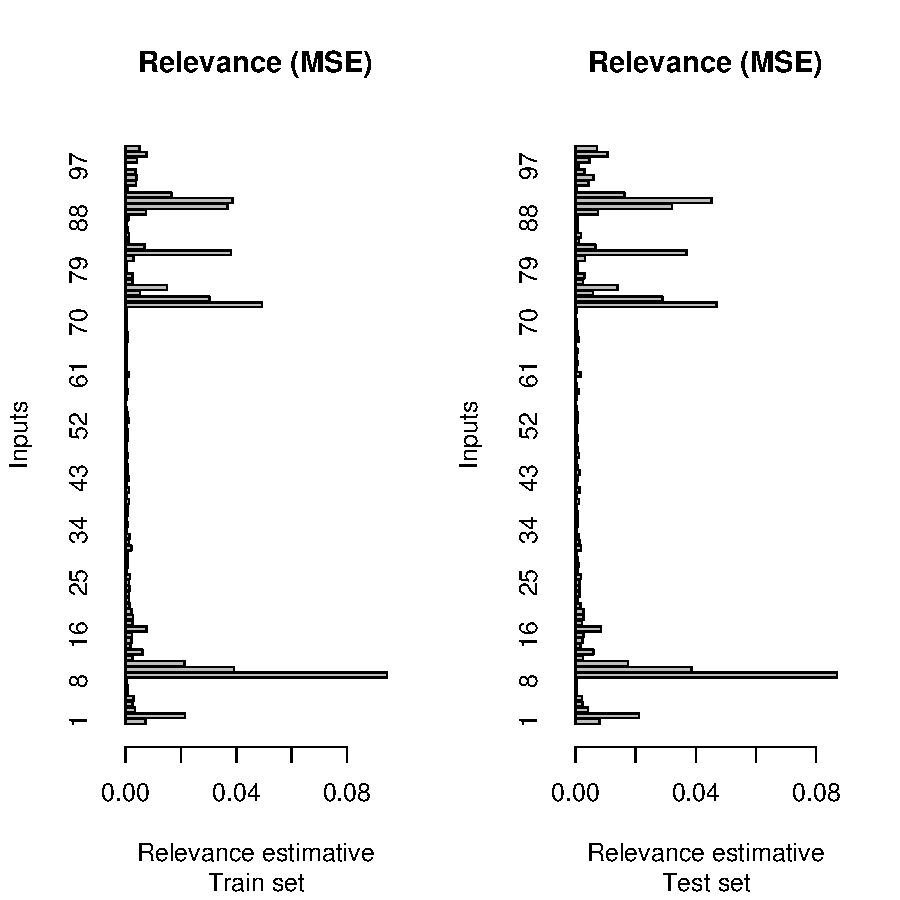
\includegraphics[scale=0.98]{t2calo-mlp-all/relevance-mse}
\end{center}
\caption{Os valores de relevância para os conjunto de treino e
teste, para as 14 variáveis do T2Calo e considerando-se o classificador neural
em estudo.}
\label{fig:t2calo-mlp-all-relevance}
\end{figure}

Aproveitando a figura de mérito utilizada para o critério de parada do
treinamento, o produto SP, seria possível desenvolver um critério de análise
de relevância que fosse compatível com o potencial discriminante de um
detetor. Ao invés de se calcular a variação do EMQ na saída do sistema, ao
fazermos uma variável assumir seu valor médio, calcula-se a variação do
produto SP na saída do detetor para as mesmas condições, assim descrita:

\begin{equation}
R_{d_i} = \max(\text{SP}_{\text{original}}) - \max(\text{SP}(\overrightarrow{x_j}\mid_{x_{j,i} = \overline{x}_i}))
\label{eq:relevance-sp}
\end{equation}

Define-se então a relevância $R_{d_i}$ da variável $i$ como a diferença
produzida no produto SP máximo no evento da substituição desta variável pelo
seu valor médio. De fato, espera-se que a maior parte dos valores de
relevância sejam positivos, indicando uma degradação do desempenho do
classificador seguindo a neutralização de uma variável. Dada a natureza do
cálculo, no entanto, é possível que se encontrem valores de relevância de
discriminação negativos, indicando que uma variável esteja, na verdade,
atrapalhando o processo de classificação ao invés de melhorá-lo. A
Figura~\ref{fig:t2calo-mlp-all-relevance-disc} mostra os valores de $R_d$ para
o classificador LMS em estudo. Como é possível ver nesta figura, o quadro é
apenas marginalmente diferente daquele mostrado pela
Figura~\ref{fig:t2calo-mlp-all-relevance}. A variável mais importante para o
processo discriminatório ainda é $\rcore$, seguindo-se de $\eratio$. É
interessante notar que o processo de análise de relevância, baseado no
conhecimento do classificador neural de melhor desempenho, indique a mesma
ordem de separação que especialistas determinam para a filtragem baseada no
EGammaHypo. O que escapa a este sistema de deteção é que existe informação
relevante para a discriminação escondida em outras variáveis que não são
contempladas pelo método, como a largura do agrupamento no calorímetro.

\begin{figure}
\begin{center}
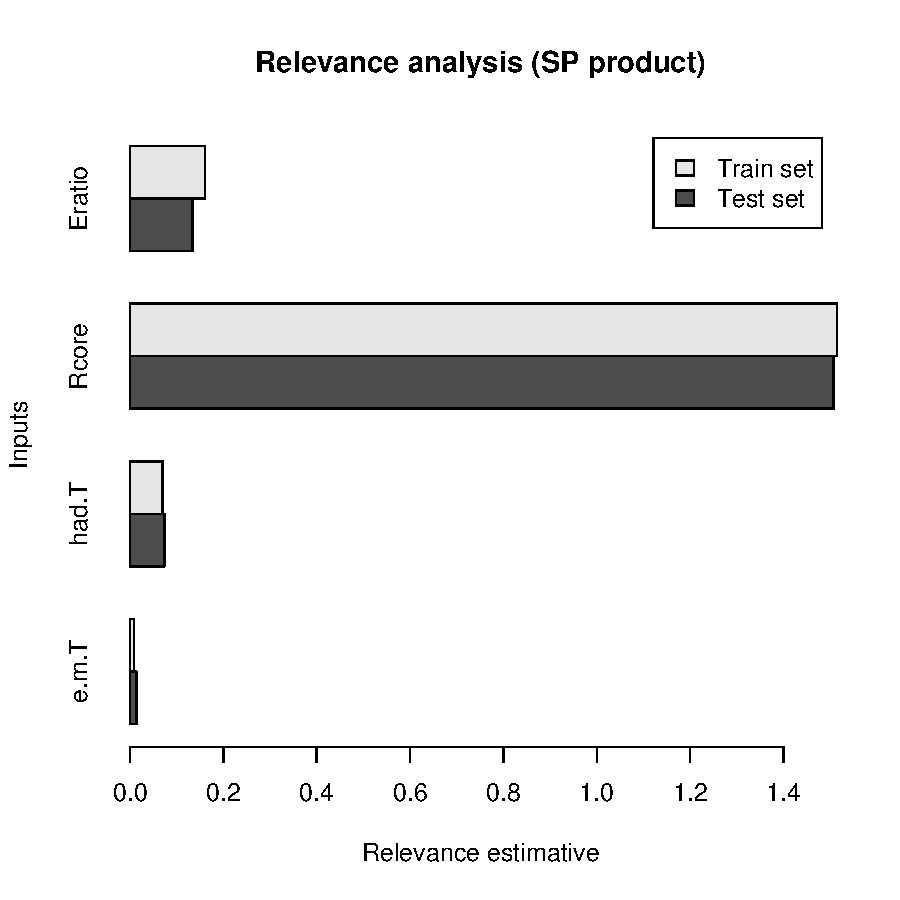
\includegraphics[scale=0.98]{t2calo-mlp-all/relevance-sp}
\end{center}
\caption{Os valores de relevância de discriminação para os conjunto de treino e
teste, para as 14 variáveis do T2Calo e considerando-se o classificador neural
em estudo.}
\label{fig:t2calo-mlp-all-relevance-disc}
\end{figure}

A análise de relevância pode ser utilizada para compactar a informação de
entrada de um detetor de forma a obter melhores desempenhos tentando-se
minimizar a perda de informação. Ao mesmo tempo, a análise de relevância pode
ser usada como medida de robustez de um sistema de deteção: quanto mais
distribuída a relevância de cada variável, menor a importância individual de
cada variável ao processo e, portanto, menor será a perda na capacidade
discriminante no caso da variável ser suprimida. A técnica de poda começa por
eliminar as variáveis que apresentam menor valor de relevância, seguindo-se
para aquelas com maior valor até que o desempenho de deteção apresente uma
degradação inaceitável ao projeto.

Para o caso em estudo, embora as relevâncias baseadas no desvio do EMQ e do
produto SP concordem, como se espera, em grande parte, na ordem de
relevância, discordam sobre a importância das variáveis entre si. Por exemplo,
a variável $\ethad$ (\texttt{had.T} nos gráficos), parece apresentar uma
importância relativa menor considerando-se a relevância baseada no desvio do
EMQ do detetor. No caso da análise da relevância discriminativa desta
variável, nota-se que ela está melhor destacada entre as 5 variáveis mais
relevantes ao processo discriminatório. De fato, uma simples poda por patamar
de corte nos dois casos, de forma a preservar as 5 variáveis mais relevantes,
escolherá conjuntos ligeiramente diferentes se nos basearmos em um ou em outro
método. Para averiguar qual dos métodos gerará um detetor mais eficiente, os
dois casos são estudados:

\begin{itemize}
\item Poda baseada na relevância pelo EMQ, preservando 5 variáveis: Rcore,
$\eratio$, largura do chuveiro (\eng{Width}), $\etem[0]$, $\etem[1]$; 
\item Poda baseada na relevância discriminativa, preservando 5 variáveis:
Rcore, $\eratio$, largura do chuveiro (\eng{Width}), $\etem[1]$, $\ethad$;
\end{itemize}

Por inspeção visual, uma poda de mais de 5 variáveis começaria a cortar
variáveis relevantes tanto ao mapeamento da entrada do sistema neural nos
alvos quanto ao poder discriminante da rede. Treinam-se 10 redes neurais para
cada um dos casos na listagem acima, observando-se os melhores resultados em
ambos. A Figura~\ref{fig:t2calo-all-relev-cut-compare} mostra curvas ROC para
os dados de testes dos melhores detetores nos dois casos. Como é possível
notar, há uma perda de eficiência de deteção do processo quando se podam 9
variáveis das 14 utilizadas pelo discriminador neural com melhor resultado. No
entanto, a poda baseada na relevância discriminativa baseada na variação do
produto SP produz melhores resultados, impedindo substancial degradação do
desempenho de classificação, como é o caso da poda pela relevância clássica.

\begin{figure}
\begin{center}
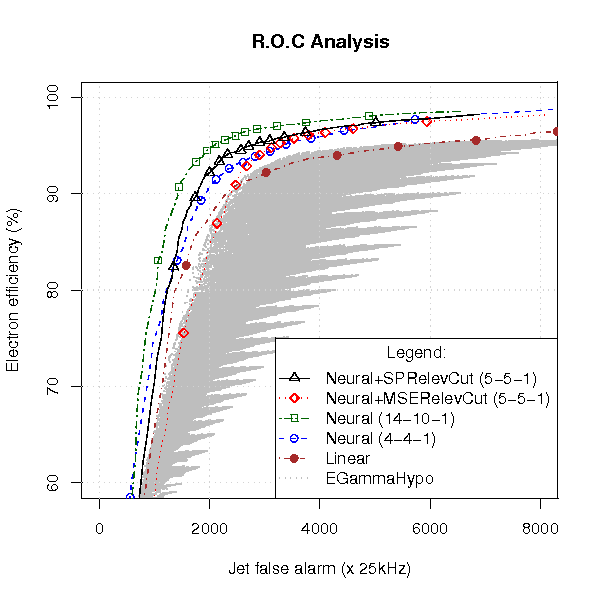
\includegraphics[scale=0.98]{t2calo-mlp-all/roc-compare-relev-cut}
\end{center}
\caption{Comparação das ROC's para os 6 detetores abordados até aqui.}
\label{fig:t2calo-all-relev-cut-compare}
\end{figure}

O classificador neural com 5 neurônios na camada de entrada, propiciado pela
poda baseada na relevância de discriminação, atinge um valor máximo para o
produto SP quando a eficiência de deteção de elétrons é igual a 93,94\% contra
9,09\% de falso-alarme na deteção de jatos. Este valor está somente cerca de 1
ponto percentual, na classificação elétrons, abaixo do valor obtido para um
classificador baseado nas 14 variáveis, para deixar passar cerca de 1,4 ponto
percentual a mais de ruído, embora conte com apenas um terço das variáveis
originais. A Figura~\ref{fig:t2calo-mlp-all-test-efficiency-eta-relev-cut-sp},
mostra outra faceta da degradação da eficiência de deteção no espaço reduzido
de variáveis gerado através da poda por relevância de discriminação. Como é
possível notar através desta figura, as perdas relativas ao \eng{crack} entre
a tampa e o barril dos calorímetros pode ser novamente identificada.

\begin{figure}
\begin{center}
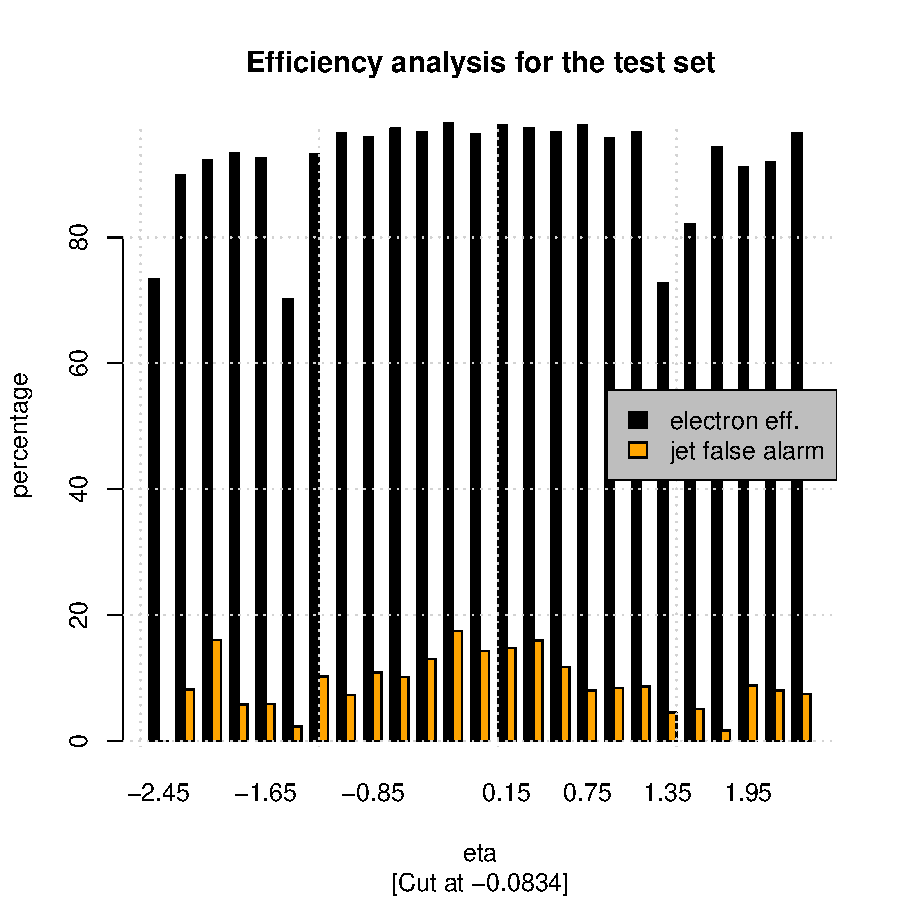
\includegraphics[scale=0.98]{t2calo-mlp-all/test-efficiency-eta-relev-cut-sp}
\end{center}
\caption{Eficiência de deteção e falso-alarme para o detetor baseado nas 5
mais relevantes (por discriminação) do espaço das 14 variáveis produzidas pelo
T2Calo.}
\label{fig:t2calo-mlp-all-test-efficiency-eta-relev-cut-sp}
\end{figure}

Das 5 variáveis de entrada selecionadas pela poda baseada na relevância
discriminativa, 3 correspondem às variáveis utilizadas pelo EGammaHypo,
escolhidas por especialistas. A análise de relevância indica que a informação
de largura do agrupamento seja mais importante à deteção que, por exemplo, a
energia total na seção e.m. dos calorímetros e, portanto, esta variável é
incluída no processo de classificação no lugar da última. A quinta variável de
interesse é a energia na primeira camada da seção e.m., que ajuda a compensar
a informação perdida ao removermos a energia total nesta seção. Este detetor é
quase tão compacto quanto o sistema T2Calo+Rede-Neural (4-4-1) e exibe uma
qualidade de discriminação compatível ou até superior (se consideramos valores
de eficiência na deteção de elétrons em patamares realísticos, i.e., acima de
80\%) a este sistema. Ainda, poupa o cálculo das energias parciais na seção
hadrônica e de algumas das camadas na seção elétromagnética. Este sistema
também evita o carregamento dos dados de energia nas camadas 0 e 3 da seção
e.m., sendo portanto mais econômico.

\subsection{Análise de Componentes Principais}

As variáveis utilizadas neste último e melhor sistema de discriminação
possuem, por sua própria natureza, uma correlação bastante elevada. Por
exemplo, há correlação entre os valores de energia totais e em cada camada de
uma determinada seção do calorímetro. Tentando aproveitar este conhecimento, é
possível encontrar, uma transformação linear (denotada por Transformação de
Kharhunen-Loève ou \gls{glos:klt}) que projeta um conjunto de variáveis em um
segundo espaço onde cada componente seja descorrelacionada de cada uma das
outra \cite{haykin}. Espera-se que operando sob o espaço transformado, onde as
variáveis são descorrelacionadas, processadores neurais consigam apresentar
melhor qualidade de separação elétron/jato e que a compactabilidade deste novo
sistema esteja mais evidente. A Figura~\ref{fig:t2calo-pca} mostra o diagrama
em blocos para este novo sistema de extração de características e deteção.

\begin{figure}
\begin{center}
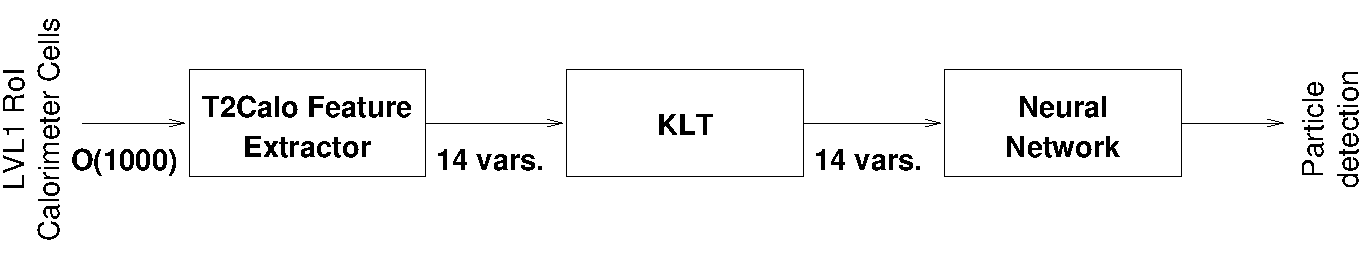
\includegraphics[scale=0.65]{t2calo-pca-block}
\end{center}
\caption{Um discriminador neural para as características definidas pela KLT
das saídas do T2Calo.}
\label{fig:t2calo-pca}
\end{figure}

Para encontramos a KLT no problema da separação elétron/jato faz-se uso do
método da covariância. A vantagem neste método é que é possível, a partir
dos autovalores da matriz de covariância, fazer diretamente uma avaliação da
energia de cada componente, o que facilitará o processo de compactação em
seguida. Para a extração baseada no método da covariância remove-se o valor
médio de cada variável de entrada baseando-se na média empírica obtida à
partir das variáveis no conjunto de treinamento, de forma a obter-se um
conjunto de entrada com média nula. Considerando:

\begin{equation}
Z = [z_1, z_2, z_3, ..., z_{14}]
\end{equation}

\noindent como o vetor de entrada, onde $z_n$ são os vetores-coluna contendo
os dados para cada uma das observações em Z, e o vetor-linha $E[Z]$ como
representativo da média (ou esperança) de cada uma das colunas:

\begin{equation}
\mathbb{E}[Z] = [\mathbb{E}[z_1], \mathbb{E}[z_2], \mathbb{E}[z_3], ...,
\mathbb{E}[z_{14}]]
\end{equation}

\noindent então podemos definir a matriz $X$, que representa $Z$ com o valor
médio de cada coluna extraído:

\begin{equation}
X = Z - [1, 1, 1, ... 1] \cdot \mathbb{E}[Z]
\end{equation}

Para encontramos a KLT de $X$, deseja-se encontrar a transformação linear $P$
de tal forma que:

\begin{align}
Y &= P^{T} \cdot X
\end{align}

\noindent com a restrição que $\text{cov}(Y)$, a covariância da matriz de
dados transformados $Y$, seja uma diagonal, isto é, não haja correlações entre
as variáveis do espaço transformado, e que $P^{-1} = P^{T}$. Por substituição:

\begin{align}
\text{cov}[Y] &= \mathbb{E}[Y \otimes Y] = \mathbb{E}[YY^{*}] \\
              &= \mathbb{E}[YY^T] = \mathbb{E}[(P^T X)(P^T X)^T] \\
              &= \mathbb{E}[(P^T X)(X^T P)] = P^T \mathbb{E}[XX^T] P \\
              &= P^T \text{cov}[X] P
\end{align}

Desta forma temos:

\begin{equation}
P\text{cov}[Y] = PP^T\text{cov}(X)P = \text{cov}[X]P
\label{eq:pca-almost}
\end{equation}

\noindent de onde finalmente, por inspeção, nota-se que, se $\text{cov}[Y]$ é
uma matriz diagonal, como se requer, então a Equação~\ref{eq:pca-almost}
assemelha-se a definição de auto-valores e auto-vetores:

\begin{equation}
V \cdot D = C \cdot V
\end{equation}

\noindent onde $V$ e $D$ representam, respectivamente, a matriz de
auto-vetores e a matriz de auto-valores de $C$. Uma vez que a matriz de
auto-vetores representa uma transformação ortonormal e que a $P^{-1} = P^T$,
então tem-se que a matriz de auto-vetores de $\text{cov}[X]$ seja a procurada
KLT. 

Para projetar uma observação (linha) do conjunto de dados $Z$, remove-se,
desta observação, o valor médio das variáveis de $Z$, em seguida
multiplicando-se o resultado pelos auto-vetores de $\text{cov}[X]$. Os
auto-valores de $\text{cov}[Y]$ são utilizados para organizar os auto-vetores
de $\text{cov}[X]$ do mais (maior auto-valor) para o menos energético,
propondo uma forma intuitiva de compactação do espaço de variáveis
transformado. Quanto maior a energia (maior o auto-valor), mais relevante a
variável seria ao processo de deteção. Esta análise por energia, conduzida
utilizando-se os auto-valores da matriz de covariância de $X$, é denominada
Análise de Componentes Principais.

A Figura~\ref{fig:t2calo-correl} mostra a correlação normalizada entre as 14
variáveis do T2Calo, com seu valor médio removido. Como é possível ver, muitas
das variáveis estão correlacionadas e portanto a Análise de Componentes
Principais pode se mostrar benéfica na procura de um discriminador mais
eficiente e compacto.

\begin{figure}
\begin{center}
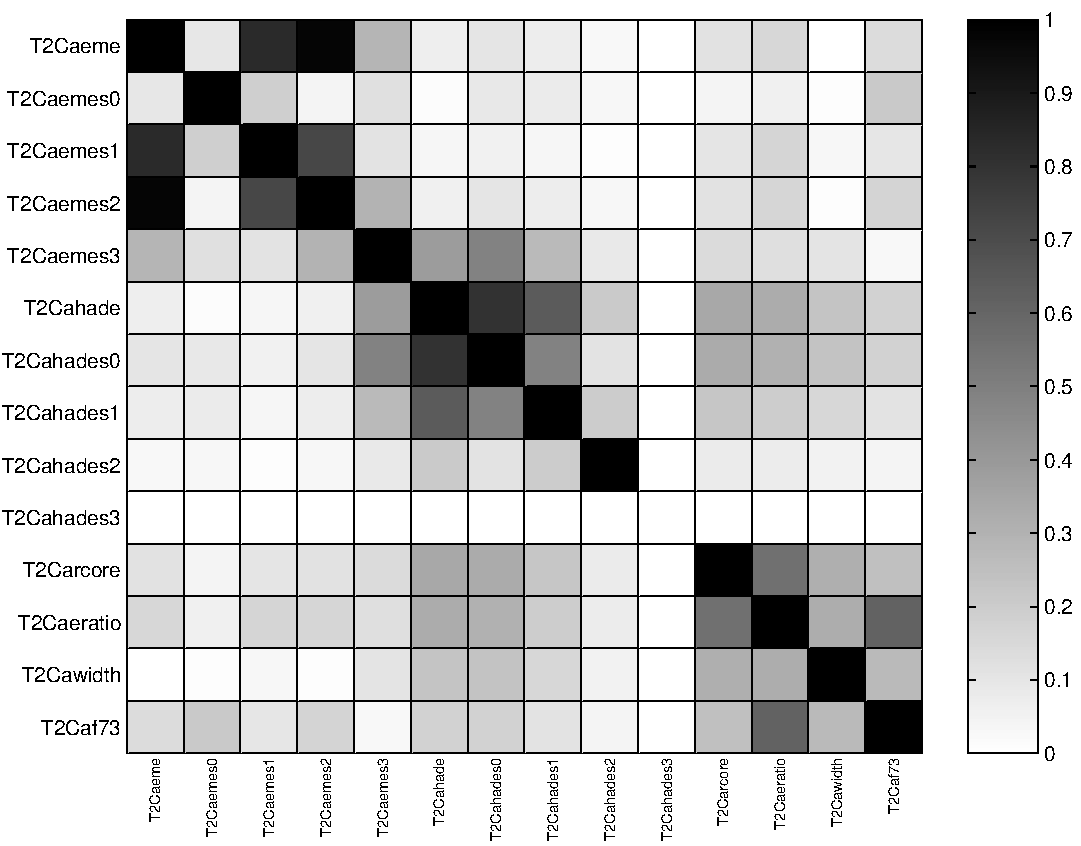
\includegraphics[scale=0.8]{t2calo-all-corr}
\end{center}
\caption{Correlação (normalizada) entre as 14 variáveis do T2Calo.}
\label{fig:t2calo-correl}
\end{figure}

Para a Análise de Componentes Principais, calculou-se o valor médio das 14
variáveis baseando-se exclusivamente nos dados do conjunto de treinamento,
utilizados também nos outros sistemas de deteção abordados até aqui. Em
seguida, através do método da covariância definido anteriormente, extraiu-se a
matriz de auto-vetores (KLT) e auto-valores (energia) baseando-se igualmente
na matriz de covariância dos dados de treinamento. A
Figura~\ref{fig:pca-charge} mostra a curva de carga em energia baseando-se no
vetor de auto-valores normalizado por sua soma. Como é possível ver, cerca de
90\% da energia total disponível é atingida com a utilização de apenas 7 das
14 variáveis no espaço transformado. As últimas 3 componentes parecem não
apresentar nenhum adicional energético ao espaço de entrada. Para uma deteção
baseada em apenas 5 das variáveis, como foi o caso da compressão atingida
empregando-se o método da compactação por relevância de discriminação na
Seção~\ref{sec:t2calo-all-relev}, apenas cerca de 73\% da energia total no
espaço transformado seria considerada.

\begin{figure}
\begin{center}
\includegraphics[scale=0.8]{t2calo-all-pca-charge}
\end{center}
\caption{A curva de carga de energia para as 14 variáveis do novo espaço
criado pela KLT.}
\label{fig:pca-charge}
\end{figure}

\subsubsection{Discriminação baseada na Análise de Componentes Principais}

Tendo por base as 14 novas variáveis do espaço provido pela PCA, é possível
definirmos um detetor neural que discrimine elétrons de jatos. Desta forma,
uma avaliação do número ideal de neurônios escondidos faz-se necessária. O
mesmo procedimento de outras seções foi tomado: treina-se 5 redes com um
número de neurônios escondidos fixo, avaliando-se a variação da eficiência de
discriminação do detetor e o tempo de treinamento até que seja automaticamente
interrompido. A Tabela~\ref{tab:t2calo-all-pca-choice} mostra os resultados
desta otimização.

\begin{table}
\caption{Resultados da otimização do número de neurônios escondidos para um
discriminador neural elétron/jato baseado na aplicação da KLT (PCA) nas 14
variáveis originais do T2Calo.}
\label{tab:t2calo-all-pca-choice}
\begin{center}
\begin{tabular}{|r|r|r|r|r|r|} \hline
N & Passos & EMQ/teste & EMQ/treino & SP/teste & SP/treino \\ \hline 
$2$ & $239\pm93$ & $0,223\pm0,004$ & $0,228\pm0,004$ & $1,601\pm0,004$ & $1,587\pm0,004$ \\
$3$ & $239\pm93$ & $0,220\pm0,004$ & $0,224\pm0,004$ & $1,605\pm0,010$ & $1,595\pm0,012$ \\
$4$ & $270\pm81$ & $0,213\pm0,003$ & $0,216\pm0,005$ & $1,614\pm0,007$ & $1,605\pm0,010$ \\
$5$ & $281\pm92$ & $0,213\pm0,004$ & $0,216\pm0,004$ & $1,612\pm0,006$ & $1,604\pm0,010$ \\
$6$ & $280\pm85$ & $0,213\pm0,004$ & $0,216\pm0,007$ & $1,617\pm0,013$ & $1,606\pm0,011$ \\
$7$ & $450\pm181$ & $0,209\pm0,004$ & $0,212\pm0,004$ & $1,625\pm0,013$ & $1,612\pm0,010$ \\
$8$ & $327\pm171$ & $0,211\pm0,004$ & $0,213\pm0,003$ & $1,617\pm0,008$ & $1,612\pm0,007$ \\
$9$ & $350\pm173$ & $0,209\pm0,002$ & $0,211\pm0,003$ & $1,622\pm0,006$ & $1,613\pm0,010$ \\
$10$ & $315\pm83$ & $0,206\pm0,004$ & $0,207\pm0,004$ & $1,630\pm0,008$ & $1,624\pm0,009$ \\
$11$ & $558\pm250$ & $0,206\pm0,007$ & $0,206\pm0,007$ & $1,631\pm0,015$ & $1,627\pm0,019$ \\
$12$ & $381\pm102$ & $0,204\pm0,002$ & $0,205\pm0,002$ & $1,641\pm0,013$ & $1,630\pm0,010$ \\
\hline
\end{tabular}
\end{center}
\end{table}

A partir desta tabela, observa-se que o número de neurônios ótimo está entre 10
e 12. Também nota-se que, comparativamente aos resultados da
Tabela~\ref{tab:t2calo-all-hidden-choice}, as médias de deteção estão
ligeiramente mais altas, atingindo $1,641$ no máximo, comparado à $1,628$ no
caso das variáveis originais do T2Calo. Escolhe-se $N=12$, treinando-se 10
redes neurais para testarmos se estas tendências são mantidas. Este exercício
é realizado com sucesso.

As Figuras~\ref{fig:pca-mse-evo} e \ref{fig:pca-sp-evo} mostram a evolução do
EMQ e do produto SP ao longo do treinamento, que neste caso dura cerca de 300
passos. Um bom grau de concordância pode ser observado entre os dois conjuntos
de dados. A ROC deste classificador pode ser vista, em comparação com aquelas
do melhor detetor baseado nas 14 variáveis originais do T2Calo, dos detetores
neural e linear baseado em apenas 4 variáveis do T2Calo e do sistema de
deteção proposto pelo EGammaHypo na Figura~\ref{fig:pca-rocs}.

\begin{figure}
\begin{center}
\includegraphics[scale=0.6]{t2calo-pca/mse-evolution}
\end{center}
\caption{Evolução do EMQ ao longo do treinamento para um classificador baseado
na KLT das 14 variáveis extraídas pelo T2Calo.}
\label{fig:pca-mse-evo}
\end{figure}

\begin{figure}
\begin{center}
\includegraphics[scale=0.6]{t2calo-pca/sp-evolution}
\end{center}
\caption{Evolução do Produto SP ao longo do treinamento para um classificador
baseado na KLT das 14 variáveis extraídas pelo T2Calo.}
\label{fig:pca-sp-evo}
\end{figure}

\begin{figure}
\begin{center}
\includegraphics[scale=0.98]{t2calo-pca/roc-pca-compare}
\end{center}
\caption{Curva ROC comparativa entre todos os métodos de deteção avaliados até
este momento e incluindo a deteção baseada em PCA.}
\label{fig:pca-rocs}
\end{figure}

O ponto onde o produto SP é máximo ($=1,64$), no caso do detetor em estudo,
apresenta uma eficiência para a deteção de elétrons de $94,75$\% contra
$7,59$\% de falso-alarme. Este novo sistema de deteção possui uma
característica de deteção bastante próxima do sistema baseado diretamente na
saída do T2Calo, usando 14 variáveis. A Figura~\ref{fig:pca-eta-phi} mostra
uma varredura da eficiência de deteção e do falso-alarme por $\eta$ e
$\phi$. Neste novo sistema, volta-se a perceber uma ligeira queda de
eficiência na deteção de elétrons próximo à região do \eng{crack}, que não era
perceptível sem a aplicação da transformação. Uma vez que a Análise de
Componentes Principais nos permite descorrelacionar totalmente a informação no
espaço projetado, e levando-se em conta que a eficiência de deteção não
aumenta significativamente a partir da utilização da KLT, conclui-se que
existem correlações de ordem mais elevada entre as 14 variáveis do T2Calo. Por
esta razão, a transformação linear provida por este método não melhora
significativamente a qualidade de deteção.

\begin{figure}
\begin{center}
\mbox{%
 \subfigure[Eficiência por $\eta$]{\includegraphics[scale=0.49]{t2calo-pca/test-efficiency-eta}}%
 \subfigure[Eficiência por $\phi$]{\includegraphics[scale=0.49]{t2calo-pca/test-efficiency-phi}}%
}
\mbox{%
 \subfigure[Produto SP por $\eta$]{\includegraphics[scale=0.49]{t2calo-pca/test-sp-eta}}%
 \subfigure[Produto SP por $\phi$]{\includegraphics[scale=0.49]{t2calo-pca/test-sp-phi}}%
}
\end{center}
\caption{Análise da eficiência de classificação e do produto SP para 
o detetor elétron/jato baseado na transformação linear (via KLT) do espaço das
14 variáveis produzidas pelo T2Calo, para os dados do conjunto de teste ao
longo de $\eta$ em (a) e (c) e por $\phi$, em (b) e (d).}
\label{fig:pca-eta-phi}
\end{figure}

%\begin{figure}
%\begin{center}
%\includegraphics[scale=0.98]{/test-efficiency-eta}
%\end{center}
%\caption{Varredura da eficiência de deteção e falso-alarme para o detetor
%elétron/jato baseado na transformação linear (via KLT) do espaço das 14
%variáveis produzidas pelo T2Calo.}
%\label{fig:pca-test-efficiency-eta}
%\end{figure}

%A Figura~\ref{fig:pca-et} mostra uma varredura da eficiência de deteção por
%energia.

%\begin{figure}
%\begin{center}
%\subfigure[Eficiência]{\includegraphics[scale=0.6]{t2calo-pca/test-efficiency-emet}}
%\subfigure[Produto SP]{\includegraphics[scale=0.6]{t2calo-pca/test-sp-emet}}
%\end{center}
%\caption{Análise da eficiência de deteção de elétrons e falso-alarme em jatos
%(a) e do produto SP (b) por $\etem$ para o detetor elétron/jato baseado na
%transformação linear (via KLT) do espaço das 14 variáveis produzidas pelo
%T2Calo, tendo por base os dados do conjunto de teste.}
%\label{fig:pca-et}
%\end{figure}

\subsubsection{Compactação baseada em PCA}

A Análise de Componentes Principais oferece um conjunto de ferramentas onde a
compactação do espaço transformado pode ser feita de forma natural. Ainda que
o detetor baseado na KLT não tenha mostrado ganho em eficiência de deteção, é
possível utilizar a informação de energia dos autovalores da matriz de
correlação para avaliar possíveis ganhos na compactabilidade do espaço das
novas 14 variáveis. A Figura~\ref{fig:pca-charge}, mostrada anteriormente,
contém a curva de carga em energia das componentes geradas por PCA. Um fato
interessante é que, com o aumento do índice da componente, a quantidade de
acréscimo em energia decai, finalmente chegando a zero, preferencialmente, em
algum ponto antes do último índice.

A análise de relevância conduzida em seções anteriores também nos oferece um
método de compactação do espaço de entrada ao sistema de deteção. Se nos
referirmos à análise de relevância de discriminação deste detetor, na
Figura~\ref{fig:pca-relevance-sp}, observaremos que, embora haja uma tendência
a haver uma diminuição da relevância com o aumento do índice da componente, a
primeira componente, que é a mais energética, é determinada como sendo uma das
menos relevantes.

\begin{figure}
\begin{center}
\includegraphics[scale=0.98]{t2calo-pca/relevance-sp}
\end{center}
\caption{Análise de relevância de discriminação para detetor baseado em uma KLT
das 14 variáveis do T2Calo.}
\label{fig:pca-relevance-sp}
\end{figure}

Para testarmos qual dos dois métodos é o mais interessante para o problema em
análise, propõe-se uma verificação em 3 podas que resultem nas mesmas
dimensões de conjuntos de dados, baseados na energia da PCA ou na análise por
relevância de discriminação\footnote{A relevância clássica demonstra as mesmas
tendências da relevância de discriminação neste caso, inclusive na ordem das
variáveis.}:

\begin{itemize}
\item Podar 3 variáveis, resultando em praticamente nenhuma perda em energia
segundo a PCA;
\item Podar 7 variáveis, resultando em aproximadamente 10\% de perda em energia
segundo a PCA;
\item Podar 9 variáveis, resultando em aproximadamente 27\% de perda em
energia segundo a PCA. Esta margem de poda também foi testada para as 14
variáveis do T2Calo na seção anterior e será possível uma comparação direta
dos dois sistemas.
\end{itemize}

Treinam-se 5 redes neurais (com inicializações diferentes) para cada uma das 6
possibilidades apresentadas acima, otimizando-se o número de neurônios
escondidos para cada uma das possibilidades. A
Tabela~\ref{tab:pca-cuts-hidden} resume os resultados da otimização do número
de neurônios escondidos para cada uma das 6 possibilidades. A coluna marcada
``Sistema'' indica o tipo de poda executada e no número de variáveis que
sobreviverão ao corte. A coluna ``N'' indica o número de neurônios escondidos
que maximiza o poder de discriminação do conjunto de entrada, baseado em 5
testes com inicializações diferentes. Os valores entre parênteses indicam
números de neurônios escondidos utilizados na varredura que culminou nos
valores otimizados desta tabela. Como é possível notar, as duas análises
apresentam tendências, no que tange à eficiência final de deteção, bastante
próximas, exceto para a última (e mais dura) poda. Neste caso, detetores
baseados na poda por relevância de discriminação apresentam resultados
nitidamente melhores. Os detetores baseados na poda por relevância também
treinam mais rapidamente, em geral. Esta tendência fica evidenciada com o
aumento do número de variáveis podadas. A
Figura~\ref{fig:roc-pca-compare-cuts} traz uma comparação das diversas ROC's
dos seis sistemas podados e do sistema de classificação baseado nas 14
componentes.

\begin{table}
\caption{Resultados da otimização do número de neurônios escondidos para um
discriminador neural elétron/jato baseado na aplicação da KLT (PCA) nas 14
variáveis originais do T2Calo.}
\label{tab:pca-cuts-hidden}
\begin{center}
\begin{tabular}{|r|r|r|r|r|} \hline
Sistema & N & Passos & EMQ/teste & SP/teste \\ \hline \hline
11 var/PCA & $6$ (2-11) & $425\pm136$ & $0,220\pm0,005$ & $1,619\pm0,014$ \\
\hline  
11 var/Rel.SP & $11$ (2-11) & $356\pm204$ & $0,220\pm0,010$ & $1,618\pm0,022$
\\ \hline  
7 var/PCA & $7$ (2-7) & $511\pm220$ & $0,233\pm0,008$ & $1,588\pm0,008$ \\
\hline  
7 var/Rel.SP & $6$ (2-7) & $258\pm125$ & $0,230\pm0,001$ & $1,595\pm0,004$ \\
\hline  
5 var/PCA & $5$ (2-5) & $181\pm67$ & $0,347\pm0,011$ & $1,443\pm0,016$ \\
\hline  
5 var/Rel.SP & $5$ (2-5) & $346\pm169$ & $0,249\pm0,004$ & $1,552\pm0,007$ \\
\hline  
\end{tabular}
\end{center}
\end{table}

\begin{figure}
\begin{center}
\includegraphics[scale=0.98]{t2calo-pca/roc-pca-compare-cuts}
\end{center}
\caption{Comparação das ROC's de diversos detetores baseados da poda (segundo
diferentes critérios) de um sistema com 14 variáveis na entrada, resultantes
da aplicação da KLT nas 14 variáveis disponíveis na saída do T2Calo.}
\label{fig:roc-pca-compare-cuts}
\end{figure}

\section{Mapeamento topológico}

Enquanto a utilização das 14 variáveis do T2Calo aplicadas a um processador
neural parece elevar o poder de discriminação do LVL2, indicando que existem
informações perdidas no processo de deteção T2Calo+EGammaHypo, pergunta-se
quanta informação é removida durante a compactação promovida pelo
algoritmo. Por outro lado, tendo-se estabelecido que sistemas de discriminação
com mais variáveis são melhores classificadores para o problema abordado,
seria possível explorar o universo de entrada original ao T2Calo, ou seja, as
células que compõem uma RoI, e se tentar recuperar mais informações sobre a
natureza da partícula.

A idéia desenvolvida nesta seção segue a seguinte linha: expande-se o número
de componentes na entrada do detetor neural, por um método que será descrito a
seguir, diminuindo-se o grau de compactação dos dados
disponíveis. Observaremos se a capacidade de deteção aumentará nestas
condições. Caso positivo, utilizaremos um estudo baseado na relevância de 
discriminação para compactar a informação de entrada de tal sistema de
deteção, a fim de obter um discriminador estruturalmente menor, ainda
guardando melhor capacidade discriminatória.

O algoritmo T2Calo, durante a análise conduzida no LVL2, compacta a informação
da RoI representando um candidato a elétron em quatro quantidades altamente
discriminantes. Embora as técnicas de deteção linear ou neurais propostas
sejam mais robustas quanto à operação e à manutenção, a qualidade física da
separação é menos afetada do que desejaríamos. Isto se deve, principalmente, à
agressiva compressão nos dados proporcionada pelo algoritmo de extração de
características. Ainda que não seja viável a deteção de objetos usando toda a
informação da RoI (cerca de 1300 células), é possível encontrar um método que
se situe a meio caminho entre estes dois extremos.

Nesta seção, propõe-se um método de compactação da informação da RoI que
utiliza a topologia do evento para gerar um conjunto de características que
pode ser usado para atingir maiores eficiências de deteção de elétrons e
menores valores de falso-alarme.

\subsection{Anelamento dos dados de uma RoI}

Observando-se a interação de elétrons e jatos (enquanto falsos-elétrons) com
os calorímetros, é possível assumir que estes objetos interagirão de forma
aproximadamente isotrópica em relação ao eixo $\eta$ do detetor. Ou seja, dado
um ponto de impacto inicial, a partícula tende a decair em objetos menos
energéticos ao redor do eixo de penetração. Este fenômeno ocorrerá de forma
expansiva, formando finalmente um cone de deposição energética, como o
exemplificado na Figura~\ref{fig:cone}.

\begin{figure}
\begin{center}
\includegraphics{msc/cone}
\end{center}
\caption{Modelo de um objeto e.m. interagindo com um calorímetro.}
\label{fig:cone}
\end{figure}

A Figura~\ref{fig:electron-roi} mostra um gráfico com a deposição energética na
segunda camada e.m. de uma RoI proveniente de um elétron simulado. As partes
acinzentadas indicam deposição energética, enquanto que as partes em branco
indicam que houve pouca ou nenhuma deposição energética na região.

\begin{figure}
\begin{center}
\includegraphics[scale=0.6]{roi-em2}
\end{center}
\caption{Imagem tridimensional mostrando a deposição energética de
um elétron simulado na segunda camada e.m. do calorímetro do ATLAS.}
\label{fig:electron-roi}
\end{figure}

Como colocado na Seção~\ref{sec:e-detection}, a topologia da interação do
objeto em análise com os calorímetros define, com boa margem de sucesso, o
tipo do mesmo. Elétrons tendem a um menor espalhamento que jatos, percorrendo
menores distâncias ao longo de $\eta$. Por outro lado, jatos tendem a
radializar a deposição energética, formando cones mais largos e possivelmente
mais profundos.

Levando-se em consideração a formatação dos calorímetros do ATLAS e sua
granularidade, sugere-se o seguinte algoritmo de compactação:

\begin{description}
\item[\ding{182}] Define-se, para cada camada, o centro de posição
energética. Isto é feito de forma simplificada, procurando para todas as
células dentro de uma mesma camada, aquela célula com maior deposição
energética;
\item[\ding{183}] Uma vez que o centro de interação esteja definido, formar um
conjunto de anéis com formato retangular que circundem este pico. A largura
destes anéis é ajustada de forma que a largura do anel de energia seja a mesma
que de uma célula dentro da camada estudada;
\item[\ding{184}] Para cada anel, somar os valores energéticos das células que
recaem sobre o seu interior.
\end{description}

Por estar adaptado ao formato da cascata energética, este método de compressão
preserva a informação da estrutura de um evento, melhor que a compactação
provida pelo T2Calo. A estrutura segmentada dos calorímetros é preservada, de
forma que tanto os valores de energia parciais quanto totais poderão ser
recuperados no final do processamento. Ainda sim, obtém-se um nível de
compressão de aproximadamente 10 vezes, sem demandar altos tempos de
processamento, como será visto no Capítulo~\ref{chap:implement}.

A Figura~\ref{fig:rings} esquematiza o algoritmo. Nesta figura, encontram-se
exemplos de anéis de energia formados em 4 diferentes camadas dos calorímetros
do detetor ATLAS. O processo de anelamento para as outras camadas é feito de
forma idêntica. Próximo ao centro da RoI, nota-se uma célula que destaca,
hipoteticamente, o centro de deposição energética conforme a etapa \ding{182}
do algoritmo viria a encontrar. Em seguida, as células de cada segmento são
somadas para a obtenção das ``características'' (somas em anel) do objeto a
ser discriminado.

\begin{figure}
\begin{center}
\includegraphics[scale=0.5]{msc/rings}
\end{center}
\caption{Esquema do processo de anelamento para as diferentes camadas
dos calorímetros do ATLAS.}
\label{fig:rings}
\end{figure}

A granularidade dos anéis respeita a granularidade \emph{típica} das células
na camada. Sabe-se, no entanto, que a granularidade das células varia com
$\eta$ no detetor. Nos casos onde a granularidade é diferente da granularidade
padrão na camada, atribuir-se-á a energia da célula ao anel onde recai o
centro da mesma. Este algoritmo também é resiliente a dados
faltantes\footnote{Ocorrendo, potencialmente, com a falha de um canal de
leitura ou do sistema de aquisição de dados.}, uma vez que células que não
puderem ser lidas apenas não serão contabilizadas. Isto evita procedimentos de
verificação especiais que poderiam comprometer o desempenho do algoritmo de
compactação proposto. Através desta figura, observa-se igualmente que algumas
camadas, devido ao formato não simétrico das células (maiores numa direção que
na outra), terão anéis abertos ou incompletos. Por isso, marcaram-se os
segmentos que pertencem ao mesmo anel com um número indicando a que anel
determinado segmento pertence.

Um problema recorrente nos algoritmos de filtragem do ATLAS é a região de
\eng{wrap-around} da variável $\phi$, já que o detetor tem formato
cilíndrico. Um cuidado especial deve ser tomado na confecção dos anéis,
levando-se em consideração que, por exemplo, a região com $\phi = 6,18$
radianos está bastante próxima a região com $\phi = 0,1$ radianos, apesar da
diferença numérica. Outro problema encontrado é que diferentes partes do
sistema de localização dos dados dentro do Athena identificam a região do
detetor onde $\phi > \pi$ de maneiras distintas. Para parte do código
(relativa à seção e.m.), o detetor se encontra na área entre $[-\pi, \pi]$
enquanto para a outra (parte hadrônica), o detetor se encontra na área entre
$[0, 2\pi]$. Para resolver este problema, implementou-se um algoritmo que
normaliza as diferenças em ambos os casos.

Ademais, por se tratar de elétrons ou jatos na qualidade de falsos-elétrons, é
bastante provável que a razão sinal-ruído seja pequena nas camadas traseiras
do detetor, principalmente na região hadrônica. A Figura~\ref{fig:roi-had-9}
mostra a deposição energética de um elétron na primeira camada do detetor
hadrônico. Nesta figura este fenômeno pode ser bem observado.

\begin{figure}
\begin{center}
\includegraphics[scale=0.6]{roi-had-9}
\end{center}
\caption{Imagem tri-dimensional mostrando a deposição energética de
um elétron simulado na primeira camada hadrônica do calorímetro do ATLAS.}
\label{fig:roi-had-9}
\end{figure}

Para evitar que o ruído inerente à eletrônica do detetor possa interferir com
a determinação do centro de deposição energética, a procura do pico em uma
camada está restrita a uma região de $\eta=0,1\times\phi=0,1$ ao redor do pico
de deposição na segunda camada e.m.. Como já colocado em um capítulo anterior
deste trabalho, a segunda camada e.m. é a mais profunda do sistema de
calorimetria, concentrando a maior parte da energia dos elétrons que interagem
com este detetor. Desta forma, se há um pico de deposição energética, este é
considerado para a formação dos anéis. De outra maneira, um ponto arbitrário
(aquele com maior energia) dentro da sub-janela definida pelo pico de
deposição energética na segunda camada e.m. é escolhido.

Tomando-se em consideração a granularidade padrão de todas as camadas do
calorímetro (7 no total, incluindo o pré-irradiador), a configuração sugerida
para o número de anéis pode ser encontrada na Tabela~\ref{tab:ring-config}. O
número de anéis em cada camada leva em consideração o número máximo de anéis
que podem ser formados, considerando-se uma sub-região de $0,4 \times 0,4$ no
plano $\eta\times\phi$, uma vez que este é o tamanho padrão da região de
interesse utilizado pelo T2Calo para a deteção de elétrons. É interessante
notar que nem sempre a região que estaria demarcada por anéis concêntricos de
uma largura determinada, excederá uma região com tamanho $0,4\times0,4$, já
que o posicionamento dos anéis dentro da RoI dependerá do centro de deposição
energética em cada camada. No entanto, uma região de $0,3\times0,3$ está
garantida ao redor do pico de energia, o que é suficiente para a análise de
elétrons \cite{daqnote00-02}.

\begin{table}
\caption{Configuração para os anéis formados a partir de uma RoI de tamanho
$\eta = 0,4 \times \phi = 0,4$.}
\label{tab:ring-config}
\begin{center}
\begin{tabular}{>{\bfseries}l r r r}
Camada & Número de Anéis & Larg. do anel ($\eta$) & Larg. do anel ($\phi$,
rad) \\ \hline
Pré-irradiador & 8 & $0,025$ & $\frac{\pi}{32} \approx 0,098174$ \\ 
1\eira\ e.m. & 64 & $0,0031245$ & $\frac{\pi}{32} \approx 0,098174$ \\ 
2\eira\ e.m. & 8 & $0,025$ & $\frac{\pi}{128} \approx 0,024544$ \\ 
3\eira\ e.m. & 8 & $0,05$ & $\frac{\pi}{128} \approx 0,024544$ \\ 
1\eira\ hadrônica & 4 & $0,1$ & $\frac{\pi}{32} \approx 0,098174$ \\ 
2\eira\ hadrônica & 4 & $0,1$ & $\frac{\pi}{32} \approx 0,098174$ \\ 
3\eira\ hadrônica & 4 & $0,1$ & $\frac{\pi}{32} \approx 0,098174$ \\ \hline
Total & 100 & & \\ \hline
\end{tabular}
\end{center}
\end{table}

Um total de $100$ anéis forma o conjunto de entrada para o novo sistema de
discriminação elétron/jato. Nota-se que o primeiro anel de cada camada será
considerado o pico de deposição energética na camada. Para classificar os
padrões neste espaço de alta dimensionalidade, utilizaremos detetores baseados
em redes neurais tipo MLP como descrito nas seções anteriores.

\subsubsection{Normalização}

Uma vez que estaremos lidando com os diferenciais energéticos dentro da mesma
camada, por muitas vezes sutis, faz-se necessário que a normalização aplicada
aos conjuntos de anéis seja compatível com a deteção destas
diferenças. Ademais, outros estudos \cite{vassali-acat-2001} já demonstraram
que a informação periférica dentro de cada camada de uma RoI é tão ou mais
importante para a discriminação que a informação de energia no centro da
RoI. Por estas razões se propõe um sistema de normalização dos dados da RoI
baseado em um conjunto de razões cujo denominador diminui, de forma
relacionada com a energia na camada, do centro para as bordas da região de
interesse. Desta forma, o pico de deposição energética na camada (ou
``primeiro anel'') teria um fator de normalização maior que o segundo anel,
que seria por sua vez maior que o fator de normalização aplicado ao terceiro
anel, e assim sucessivamente. O algoritmo está anotado na
Tabela~\ref{tab:seq}.

\begin{table}
\renewcommand{\baselinestretch}{1.5}
\caption{Algoritmo para a ``Normalização Seqüencial''.}
\label{tab:seq}
\renewcommand{\baselinestretch}{1}
\begin{center}
\begin{tabular}{>{\bfseries}l r r}
Anel & Fator de Normalização & Soma em anel \\ \hline
1 & $E$ (total da camada) & $E_1$\\
2 & $E - E_1$ & $E_2$ \\
3 & $E - E_1 - E_2$ & $E_3$\\
4 & $E - E_1 - E_2 - E_3$ & $E_4$\\
\dots  & \dots \\
N-4 & $E - E_1 - E_2 - ... - E_{N-5}$ & $E_{N-4}$ \\
N-3 & $E - E_1 - E_2 - ... - E_{N-5} - E_{N-4}$ & $E_{N-3}$ \\
N-2 & $E - E_1 - E_2 - ... - E_{N-4} - E_{N-3}$ & $E_{N-2}$ \\
N-1 & $E - E_1 - E_2 - ... - E_{N-3} - E_{N-2}$ & $E_{N-1}$ \\
N & $E - E_1 - E_2 - ... - E_{N-2} - E_{N-1}$ & $E_N$ \\
\end{tabular}
\end{center}
\end{table}

Neste algoritmo, o primeiro anel (pico de deposição energética) será
normalizado pelo valor da energia total na camada. O segundo anel pelo valor
da camada subtraindo-se o valor de deposição energética no primeiro anel. O
terceiro anel, pelo valor da energia na camada menos o valor do primeiro e
segundo anéis, e desta forma recursivamente, até que todos os anéis estejam
normalizados. Referir-nos-emos à este algoritmo a partir de agora como
algoritmo de ``Normalização Seqüencial''.

Nota-se que este tipo de normalização poderá amplificar em demasiado os
valores periféricos. Isto é desejável para os anéis que se sucedem ao pico de
energia na camada, porém nem tanto para os anéis da periferia da RoI, mais
distantes, onde a razão sinal-ruído é praticamente nula. Desta forma,
propõe-se que, a partir de um determinado limiar de energia, o fator de
normalização torne-se constante. Desta forma evita-se que o sinal ruidoso das
bordas influencie o sistema de discriminação de maneira significativa.

O sub-pacote \texttt{rbuild} do \eng{NeuralRinger} contém a implementação de
referência para este processo de anelamento descrito (ver
Apêndice~\ref{ap:framework}). Ademais, este pacote pode ser reconfigurado de
forma a definir a largura dos anéis de cada camada ou o número máximo de anéis
por camada. Assim, o sistema de anelamento torna-se independente do tamanho
real da RoI e, portanto, independente de quão completos são os dados recebidos
pelo processador do LVL2. Anéis sem dados recebem o valor \eng{default}, que é
igual a zero. O formato do arquivo de configuração é também XML, o que
simplifica a leitura e escrita dentro do contexto do trabalho.

\subsubsection{Dados}

Os dados em seu formato utilizado nas seções anteriores não podem ser
re-aproveitados para esta porção do projeto, uma vez que necessita-se do
acesso aos dados ``brutos'' da RoI. Em outras palavras, deseja-se acesso aos
mesmos dados utilizados pelo T2Calo para a operação de extração de
características que este algoritmo realiza. De posse destes dados, será
possível definir a operação de compactação topológica proposta. A
Figura~\ref{fig:datagen} mostra o sistema que foi utilizado para a obtenção
dos dados. Para cada RoI que é analisada pelo T2Calo, um conjunto de células é
carregado dos arquivos de dados iniciais. Em seguida, os valores das células
são calibrados e mapeados na geometria do detetor de forma que possam ser mais
facilmente acessados pelo algoritmo de extração de características. A partir
deste ponto, o T2Calo tem acesso aos dados e, é exatamente neste ponto que
inserimos um \eng{patch}, que permite que os valores das células ``vistas''
pelo algoritmo sejam guardados em um arquivo separado.

\begin{figure}
\begin{center}
\includegraphics[scale=0.74]{datagen}
\end{center}
\caption{Estratégia para obter acesso aos dados tais como processados pelo
algoritmo T2Calo.}
\label{fig:datagen}
\end{figure}

O formato deste arquivo é legível pelo sub-pacote \texttt{roiformat} do
\eng{NeuralRinger} e pode ser transformado em uma base de dados de anéis
utilizando-se o programa \texttt{ringer}, descrito no
Apêndice~\ref{ap:framework}. Desta forma, criou-se uma base de dados a partir
do mesmo conjunto de eventos analisados na caracterização do desempenho físico
do T2Calo. Esta nova base de dados tem cerca de $30000$ eventos com a mesma
proveniência e características dos eventos analisados até o momento.

\subsection{Discriminação baseada em anelamento}

A Figura~\ref{fig:ringer-neural} mostra o diagrama de blocos do novo sistema
de deteção elétron/jato proposto. Neste caso, substitui-se o bloco de extração
de características pelo extrator em anéis. O processo de anelamento reduz o
espaço de dados de entrada em uma RoI (cerca de 1300 células) para 100 valores
correspondentes aos anéis formados com os dados das 7 camadas dos
calorímetros. Adota-se um sistema de discriminação neural, conectado à saída
do sistema de anelamento, que executará o processo de deteção.

\begin{figure}
\begin{center}
\includegraphics[scale=0.8]{ringer-neural}
\end{center}
\caption{Diagrama em blocos de um sistema de deteção utilizando o anelador
como extrator de características e um detetor neural.}
\label{fig:ringer-neural}
\end{figure}

Tal qual nos sistemas anteriores, executou-se uma análise do número de
neurônios ótimo para a camada escondida. Um cuidado deve ser tomado: com o
aumento de neurônios no nó de entrada do discriminador neural, o número de
parâmetros livres, que se deseja sintonizar, aumenta bruscamente. Finalmente,
deve ser levando em consideração que cerca de 3500 jatos são usados para
treinamento do sistema. Considerando-se $N$, o número de neurônios na camada
escondida do discriminador neural, o número de parâmetros livres ($K$) a serem
treinados pode ser computado da seguinte forma:

\begin{align}
K &= (100 \times N) + N \text{(polarização)} + N 
\text{(con. saída)} + 1 \text{(pol. saída)} \\
&= (102 \times N) + 1
\end{align}

Desta forma, para, por exemplo, 12 neurônios na camada escondida, o número de
parâmetros livres é 1225; para 11, 1123 e para 10, 1003. Estes números estão
próximos de um limite sensível para o treinamento do sistema e, desta forma,
limitar-nos-emos a este patamar (12 neurônios escondidos). Portanto, varia-se o
número de neurônios escondidos entre 2 e 12. A
Tabela~\ref{tab:ringer-param-optimization} resume os resultados, indicando o
número de neurônios escondidos utilizados e os resultados para cada agrupamento
de teste.

\begin{table}
\caption{Análise dos parâmetros de treinamento para um detetor neural cuja
entrada são os 100 anéis resultantes do processamento de uma RoI.}
\label{tab:ringer-param-optimization}
\begin{center}
\begin{tabular}{|r|r|r|r|r|r|} \hline
N & Passos & EMQ/teste & EMQ/treino & SP/teste & SP/treino \\ \hline 
$2$ & $242\pm59$ & $0,133\pm0,002$ & $0,098\pm0,002$ & $1,763\pm0,005$ &
$1,821\pm0,008$ \\ 
$3$ & $473\pm128$ & $0,129\pm0,003$ & $0,089\pm0,004$ & $1,764\pm0,006$ & $1,840
\pm0,011$ \\
$4$ & $654\pm283$ & $0,123\pm0,004$ & $0,079\pm0,002$ & $1,781\pm0,011$ & $1,861
\pm0,007$ \\
$5$ & $531\pm124$ & $0,124\pm0,006$ & $0,077\pm0,005$ & $1,774\pm0,012$ & $1,864
\pm0,011$ \\
$6$ & $808\pm220$ & $0,124\pm0,003$ & $0,070\pm0,004$ & $1,776\pm0,007$ & $1,877
\pm0,012$ \\
$7$ & $898\pm217$ & $0,124\pm0,003$ & $0,065\pm0,004$ & $1,777\pm0,008$ & $1,890
\pm0,006$ \\
$8$ & $910\pm340$ & $0,122\pm0,005$ & $0,063\pm0,004$ & $1,777\pm0,012$ & $1,894
\pm0,008$ \\
$9$ & $930\pm207$ & $0,120\pm0,004$ & $0,060\pm0,003$ & $1,780\pm0,010$ & $1,900
\pm0,006$ \\
$10$ & $1426\pm453$ & $0,120\pm0,002$ & $0,054\pm0,002$ & $1,782\pm0,009$ & $1,9
10\pm0,002$ \\
$11$ & $990\pm343$ & $0,120\pm0,002$ & $0,055\pm0,002$ & $1,782\pm0,006$ & $1,90
8\pm0,004$ \\
$12$ & $930\pm240$ & $0,116\pm0,004$ & $0,050\pm0,003$ & $1,785\pm0,007$ & $1,91
8\pm0,006$ \\
\hline
\end{tabular}
\end{center}
\end{table}

Através desta tabela, nota-se que o número mínimo de neurônios na camada
escondida deve ser maior ou igual a 4, já que a partir deste número o
desempenho da rede melhora tanto com relação ao mapeamento da entrada nos
alvos de treinamento (EMQ menor) quanto com relação ao poder
discriminante. Quando $N=12$ o sistema aparenta atingir um máximo, registrando
a menor média para o EMQ do conjunto de testes, com baixo desvio assim como
bons patamares de deteção. O número de épocas de treinamento é maior a partir
de $N=6$, chegando a ser bem maior que 1000 quando $N=10$. Desta forma,
escolhe-se $N=12$.

\subsubsection{Resultados para o \eng{NeuralRinger}}

Baseando-se no número de neurônios destacado anteriormente, treinaram-se dez
redes que tiveram seus pesos sinápticos iniciais fixados em valores aleatórios
(no intervalo $[-1,+1]$) e diferentes para cada uma destas iterações. A
Figura~\ref{fig:ringer-mlp-mse} mostra a evolução do EMQ da rede com melhor
desempenho discriminatório. A Figura~\ref{fig:ringer-mlp-sp} mostra um gráfico
equivalente para a evolução do produto SP ao longo do treinamento da
rede. Como é possível distinguir, após cerca de 100 passos de treinamento a
capacidade discriminante da rede para o conjunto de teste estagna. A
capacidade de mapeamento nos alvos (medido pelo EMQ) da rede, com relação ao
conjunto de treinamento, apesar da estagnação do conjunto de teste, ainda
continua a melhorar após os 100 passos, chegando, no momento onde o treinamento
é automaticamente interrompido, a um valor de pouco menor que $0,05$,
indicando um produto SP de $1,91$. Ainda assim, não se observa, para o sistema
em análise (também levando em consideração os outros 9 testes), o fenômeno
conhecido como \eng{overtraining}, onde a capacidade de generalização da rede
é penalizada por uma excessiva especialização no conjunto de treino,
normalmente fazendo com que ocorra um aumento no EMQ do discriminador para o
conjunto de teste.

\begin{figure}
\begin{center}
\includegraphics[scale=0.6]{ringer-mlp/mse-evolution}
\end{center}
\caption{Evolução do EMQ para os conjuntos de treino e teste de um
discriminador elétron/jato neural para as variáveis do anelador.}
\label{fig:ringer-mlp-mse}
\end{figure}

\begin{figure}
\begin{center}
\includegraphics[scale=0.6]{ringer-mlp/sp-evolution}
\end{center}
\caption{Evolução do produto SP para os conjuntos de treino e teste de um
discriminador elétron/jato neural para as variáveis do anelador.}
\label{fig:ringer-mlp-sp}
\end{figure}

A Figura~\ref{fig:ringer-mlp-output} contém a saída da rede após o treinamento
do detetor neural. Diferente dos casos anteriores, o sistema parece
identificar com bastante precisão elétrons e jatos, mostrando nítidas
``torres'' de concentração de eventos nos pólos do gráfico. Um corte em
$-0,07$ estabelece o máximo do produto SP (conjunto de teste) para esta rede,
com uma eficiência de $96,21$\% na deteção de elétrons contra apenas $3,44$\%
de falso-alarme em jatos. O produto SP para estes valores é $\approx 1,79$,
representando o melhor valor para este índice obtido até o momento. Este valor
está $0,16$ ponto acima do valor obtido para um detetor neural baseado em
todas as características extraídas pelo T2Calo, $0,25$ ponto acima do valor
obtido para as 4 saídas (de discriminação) do T2Calo usando um detetor neural
e $0,31$ ponto (do produto SP) para um detetor baseado no algoritmo LMS! Em
termos de rejeição de ruído, este novo sistema apresenta-se cerca de 6 vezes
melhor que o proposto pela combinação do T2Calo aliado à discriminação
utilizando o algoritmo EGammaHypo.

\begin{figure}
\begin{center}
\includegraphics[scale=0.98]{ringer-mlp/test-output}
\end{center}
\caption{Saída para o conjunto de teste, do discriminador neural baseado nas
características extraídas pelo anelador.}
\label{fig:ringer-mlp-output}
\end{figure}

A Figura~\ref{fig:ringer-test-roc} contém uma comparação das R.O.C. entre
todos métodos estudados até o momento. Como é possível perceber, o método
proposto de anelamento, associado a um detetor neural produz um resultado
significativamente melhor para a massa de dados avaliada. Para um mesmo valor
de eficiência na deteção de elétrons, por exemplo $90$\%, o sistema baseado no
anelador aprovará apenas cerca de 400~Hz em jatos ao passo que o sistema
baseado na solução atual (EGammaHypo) para o LVL2, cerca de 2,4~kHz. Por outro
ângulo este resultado traz que, para uma mesma capacidade de aprovar elétrons,
um sistema baseado no anelamento e redes neurais poupará 6 vezes mais o
terceiro nível de filtragem do experimento ATLAS. Se, por outro lado, deseja-se
aumentar a eficiência na deteção de elétrons, o anelador consegue, até cerca
de $96$\% de eficiência, manter uma taxa de falso-alarme igual ou inferior a
1~kHz. Para o sistema atual baseado no EGammaHypo, para uma eficiência na
deteção de elétrons de $97$\%, $100$\% dos jatos deveriam ser aprovados, o que
seria inviável.

\begin{figure}
\begin{center}
\includegraphics[scale=0.98]{ringer-mlp/roc-compare}
\end{center}
\caption{Comparação da R.O.C. dos diversos sistemas de filtragem abordados até
agora com o sistema neural baseado em anéis de deposição energética.} 
\label{fig:ringer-test-roc}
\end{figure}

A Figura~\ref{fig:ringer-eta-phi} mostra os valores do produto SP por
intervalo em $\eta$ e em $\phi$. Observa-se neste caso que a recuperação do
sinal perdido na região do \eng{crack} é excelente, sendo difícil notar onde
realmente ocorre, o que pode ser facilmente percebido nos outros métodos. Na
parte central do detetor, onde a maior parte dos eventos de interesse se
concentrarão, o valor do produto SP é bastante alto, chegando, em alguns
pontos, a aproximar-se de $2,0$. A eficiência de deteção para elétrons é de
praticamente 100\% nesta região. O gráfico equivalente em $\phi$ mostra a
homogeneidade esperada para todo o espectro.

\begin{figure}
\begin{center}
\mbox{%
 \subfigure[Eficiência por $\eta$]{\includegraphics[scale=0.49]{ringer-mlp/test-efficiency-eta}}%
 \subfigure[Eficiência por $\phi$]{\includegraphics[scale=0.49]{ringer-mlp/test-efficiency-phi}}%
}
\mbox{%
 \subfigure[Produto SP por $\eta$]{\includegraphics[scale=0.49]{ringer-mlp/test-sp-eta}}%
 \subfigure[Produto SP por $\phi$]{\includegraphics[scale=0.49]{ringer-mlp/test-sp-phi}}%
}
\end{center}
\caption{Análise da eficiência de classificação e do produto SP para o
discriminador neural baseado nas saídas do anelador, para os dados do conjunto
de teste ao longo de $\eta$ em (a) e (c) e por $\phi$, em (b) e (d).}
\label{fig:ringer-eta-phi}
\end{figure}

%\begin{figure}
%\begin{center}
%\includegraphics[scale=0.98]{ringer-mlp/test-sp-eta}
%\end{center}
%\caption{Análise do produto SP ao longo de $\eta$ para o discriminador neural
%baseado nas saídas do anelador.}
%\label{fig:ringer-test-sp-eta}
%\end{figure}

%\begin{figure}
%\begin{center}
%\includegraphics[scale=0.98]{ringer-mlp/test-sp-phi}
%\end{center}
%\caption{Análise do produto SP ao longo de $\phi$ para o discriminador neural
%baseado nas saídas do anelador.}
%\label{fig:ringer-test-sp-phi}
%\end{figure}

A Figura~\ref{fig:ringer-efficiency-et} contém uma análise da eficiência de
deteção (a) e do produto SP (b) por intervalo em $\etem$. A eficiência de
deteção neste caso apresenta-se aproximadamente constante, até a faixa de
energia em torno de 100~GeV, caindo abruptamente em seguida. Os números no
topo de cada barra indicam a quantidade de elétrons e jatos analisadas no
intervalo e servem como uma medida da significância do resultado. Para valores
de energia acima de $\approx 100$~GeV, o número de eventos disponíveis para
treino e análise cai significativamente, devido à natureza dos eventos
estudados. Por esta razão, os resultados para altos valores energéticos devem
ser considerados com esta ressalva. A Figura~\ref{fig:ringer-et-compare} traz
uma comparação da capacidade discriminativa deste novo sistema, com os métodos
de discriminação neurais baseados na saída do T2Calo (parcial, com 4 variáveis
e completa com 14 variáveis). Este novo sistema possui melhor discriminação
nas faixas de energia com mais eventos, superando em muitos pontos os outros
dois detetores.

\begin{figure}
\begin{center}
\subfigure[Eficiência]{\includegraphics[scale=0.6]{ringer-mlp/test-efficiency-emet}}
\subfigure[Produto SP]{\includegraphics[scale=0.6]{ringer-mlp/test-sp-emet}}
\end{center}
\caption{Análise da eficiência de deteção de elétrons e falso-alarme em jatos
(a) e do produto SP (b) por $\etem$ para o discriminador neural baseado nas
saídas do anelador, tendo por base os dados do conjunto de teste.}
\label{fig:ringer-efficiency-et}
\end{figure}

\begin{figure}
\begin{center}
\includegraphics[scale=0.98]{ringer-mlp/et-compare}
\end{center}
\caption{Gráfico comparativo do produto SP ao longo de $E^{e.m.}_T$ para os
discriminador neurais baseados nas saídas do anelador, parcial e completa do
T2Calo.}
\label{fig:ringer-et-compare}
\end{figure}

As Figuras~\ref{fig:ringer-mse-relevance} e \ref{fig:ringer-sp-relevance}
trazem as análises de relevância para o conjunto de teste, das 100 variáveis
do anelador, tendo em vista a variação do EMQ e do produto SP
respectivamente. Os dois gráficos parecem indicar, igualmente, uma grande
importância nos primeiros anéis de cada camada (veja
Tabela~\ref{tab:ringer-position}). A importância de cada anel diminui, em
geral, com o afastamento do centro, onde pressupõe-se que a razão sinal ruído
seja inferior. A importância relativa entre os anéis mais importantes e
aqueles de menor importância parece ser menor da perspectiva da relevância
baseada no produto SP que da relevância clássica, como também observado na
análise das 14 variáveis produzidas pelo T2Calo. Outra informação que pode ser
aferida é a importância da informação na primeira camada e.m.. Para a
relevância clássica, as variáveis desta camada constituem uma informação
essencial na determinação da saída, indicando ser duas vezes mais relevantes
que os dados de outras camadas. Na avaliação baseada na capacidade
discriminante do sistema, a parte hadrônica é a mais importante, sobretudo a
primeira camada indica ser a mais relevante. É interessante notar mais uma vez
que a informação de relevância está ligada diretamente ao caráter físico do
evento: para a discriminação, os valores mais relevantes na deteção
elétron/jato são, sem dúvida, a informação de depósito de energia ao longo das
camadas e, em especial, a existência de energia na primeira camada hadrônica,
indicando que o evento contenha componentes desta natureza (aumentando a
probabilidade de não ser um elétron). O detetor baseado nos anéis de deposição
energética ``aprende'' este conceito através da análise do conjunto de dados,
sem a necessidade da intervenção de um especialista.

\begin{figure}
\begin{center}
\includegraphics[scale=0.98]{ringer-mlp/relevance-mse}
\end{center}
\caption{Os valores de relevância para os conjunto de teste, para as 100
variáveis do anelador e considerando-se o classificador neural em estudo, como
indica a Tabela~\ref{tab:ringer-position}.} 
\label{fig:ringer-mse-relevance}
\end{figure}

\begin{figure}
\begin{center}
\includegraphics[scale=0.98]{ringer-mlp/relevance-sp}
\end{center}
\caption{Os valores de relevância de discriminação para os conjunto de teste,
para as 100 variáveis do anelador e considerando-se o classificador neural em
estudo, como indica a Tabela~\ref{tab:ringer-position}.}
\label{fig:ringer-sp-relevance}
\end{figure}

\begin{table}
\caption{Posicionamento relativo dos anéis produzidos pelo anelador no vetor
de entrada ao sistema de deteção neural.}
\label{tab:ringer-position}
\begin{center}
\begin{tabular}{|l|r|r|r|} \hline
\textbf{Camada} & \textbf{Número de anéis} & \textbf{Primeiro} &
\textbf{Último} \\ \hline
Pré-irradiador & 8 & 1 & 8 \\
1\eira e.m. & 64 & 9 & 72 \\
2\eira e.m. & 8 & 73 & 80 \\
3\eira e.m. & 8 & 81 & 88 \\
1\eira hadrônica & 4 & 89 & 92 \\
2\eira hadrônica & 4 & 93 & 96 \\
3\eira hadrônica & 4 & 97 & 100 \\ \hline
\end{tabular}
\end{center}
\end{table}

\subsection{Compactação baseada na relevância}

A informação de relevância estudada até aqui pode ser aproveitada para que se
aplique sobre as entradas do discriminador neural uma poda baseada na
capacidade discriminante de uma variável. Esta poda pode ser feita
automaticamente \cite{aa:enfpc-00} em muitos casos, ou manualmente, se forem
necessárias otimizações no processo de poda.

Um fator interessante e novo até o momento é o aparecimento de valores
negativos de relevância, cuja possibilidade havia sido prevista
anteriormente. Esta informação indica que existem variáveis que dificultem o
treinamento da rede e, por conseqüência, o processo de discriminação
proporcionado pela combinação anelador $+$ redes neurais. Para validarmos esta
tendência, eliminam-se do conjunto de treinamento e testes as variáveis com
relevância de discriminação negativas, aplicando-se um patamar de poda em $0$
(zero). Neste modo, 62 variáveis sobrevivem ao corte, como indicado na
Tabela~\ref{tab:cut-negative-relev}.

\begin{table}
\caption{Anéis sobreviventes de uma poda baseada na relevância de discriminação.}
\label{tab:cut-negative-relev}
\begin{center}
\begin{tabular}{|l|r|r|r|r|} \hline
\textbf{Camada} & \textbf{Número de anéis} & \textbf{Primeiro} &
\textbf{Último} & \textbf{Anéis removidos}\\ \hline
Pré-irradiador & 6 & 1 & 6 & 2\\
% REM: 4, 8
% STAY: 1, 2, 3, 5, 6, 7 (6)
1\eira e.m. & 36 & 7 & 42 & 28\\
% REM: 14,16,22,33-36,38,40-45,47,50,51,54,58,61,64,65,67-72, TOTAL = 28
% STAY: 9-13 (5), 15, 17-21 (5), 23-32 (10), 37, 39, 46, 48, 49, 52, 53, 
% 55-57(3), 59, 60, 62, 63, 66, TOTAL = 36
2\eira e.m. & 5 & 43 & 47 & 3 \\
% REM: 76-78 (3)
% STAY: 72-75, 79 (5)
3\eira e.m. & 5 & 48 & 52 & 3 \\
% REM: 85-87 (3)
% STAY: 80-84 (5)
1\eira hadrônica & 4 & 53 & 56 & 0\\
% REMAINS THE SAME
2\eira hadrônica & 3 & 57 & 59 & 1\\ 
% REM: 93 (1)
% STAY: 94-96 (3)
3\eira hadrônica & 3 & 60 & 62 & 1\\ \hline
% REM: 97 (1)
% STAY: 98-100 (3)
\end{tabular}
\end{center}
\end{table}

Nota-se que a camada que teve mais cortes foi a 1\eira camada e.m.. Esta
camada tem uma geometria de células muito particular: 4 vezes mais compridas
ao longo da variável $\phi$ e 8 vezes mais finas ao longo de $\eta$,
comparativamente à 2\eira camada e.m.. Ela é utilizada para detetar a
multiplicidade da cascata, indicando a presença de muitas partículas ao invés
de apenas uma.  A informação de deteção entre elétrons e jatos encontra-se,
naturalmente, próxima ao centro da RoI para esta camada, uma vez que elétrons
(partículas simples) exibirão um pico de deposição energética pronunciado nos
arredores do centro, ao passo que jatos, na qualidade de falsos-elétrons,
vários picos situados também nesta região. Caso esta afirmação não fosse
verdadeira, o LVL1 provavelmente não teria selecionado o evento, pois a RoI
não passaria o teste de isolamento em energia na seção e.m.. Desta forma, como
é esperado, o sistema de deteção indica que os anéis na parte exterior (em sua
maioria) sejam pouco relevantes ao processo discriminatório, dificultando o
processo de aprendizado do detetor neural.

No caso das outras camadas, as informações da periferia mais distante são
consideradas menos relevantes, como é de se esperar. Isto não quer dizer, em
absoluto, que a informação periférica não seja importante. Quer dizer,
simplesmente que, muito longe do centro, chega-se a um ponto onde não existe
mais interação da partícula com o detetor, e portanto a informação contida
nesta região não ajuda a discrimina\c{c}ão.

De posse dos 62 anéis que sobreviveram ao corte de discriminação, treinam-se
10 redes neurais, ainda com 12 neurônios escondidos, partindo-se de
inicializações distintas. Observa-se a variabilidade de parâmetros como o
número de épocas necessárias ao treinamento (espera-se que convirja mais
rápido) e os valores finais de EMQ e produto SP que se espera, sejam maiores
que no caso anterior utilizando-se os 100 anéis. Em média, este novo sistema
toma cerca de 552 passos de treinamento para atingir a estagnação do produto
SP. O desvio-padrão para o número de passos de treinamento é de apenas 130
passos, indicando boa concordância entre os detetores destes últimos testes,
no que tange este aspecto; sobretudo em comparação ao sistema anterior, onde
observaram-se $930\pm240$ passos de treinamento. O EMQ do conjunto de teste
cai ligeiramente, na média, passando de $0,116\pm0,004$ para
$0,110\pm0,002$. O produto SP de teste aumenta 0,032 ponto, passando de
$1,785\pm0,007$ para $1,807\pm0,004$. O produto SP máximo determina uma
eficiência na deteção de elétrons de 96,64\% contra apenas 3,17\% de
falso-alarme. A Figura~\ref{fig:ringer-mlp-relev-cut-0-roc} mostra uma
comparação das ROC's de alguns do discriminadores analisados até o momento.

\begin{figure}
\begin{center}
\includegraphics[scale=0.98]{ringer-mlp/roc-compare-relev-cut-0}
\end{center}
\caption{Comparação entre as ROCs de alguns dos sistemas de discriminação
abordados até aqui. Em destaque, a ROC do melhor discriminador (linha cheia),
determinado a partir da análise de relevância.}
\label{fig:ringer-mlp-relev-cut-0-roc}
\end{figure}

A Figura~\ref{fig:ringer-mlp-relev-cut-0-relev} traz, mais uma vez, a análise
de relevância de discriminação do sistema baseado em 62 dos 100 anéis
originais. Como é possível determinar, ainda existem cerca de 14 componentes
que apresentam relevância negativa. Um segundo corte baseado nesta observação
será realizado. A Tabela~\ref{tab:cut-negative-relev-1} contém a informação
dos anéis sobreviventes. Após reajustar os pesos sinápticos, o discriminador
neural, mais uma vez tende a remover anéis excedentes da periferia da 1\eira
camada e.m.. O número total de anéis neste momento é menor que metade dos
anéis originais.

\begin{figure}
\begin{center}
\includegraphics[scale=0.98]{ringer-mlp/relevance-sp-cut-0}
\end{center}
\caption{Os valores de relevância de discriminação para os conjunto de treino
e teste, para as 62 variáveis que sobreviveram a uma poda baseada na
relevância de discriminação.}
\label{fig:ringer-mlp-relev-cut-0-relev}
\end{figure}

\begin{table}
\caption{Anéis sobreviventes de uma segunda poda baseada na relevância de
discriminação.} 
\label{tab:cut-negative-relev-1}
\begin{center}
\begin{tabular}{|l|r|r|r|r|} \hline
\textbf{Camada} & \textbf{Número de anéis} & \textbf{Primeiro} &
\textbf{Último} & \textbf{Anéis removidos}\\ \hline
Pré-irradiador & 6 & 1 & 6 & 0\\ %0
% REMAINS THE SAME AS THE PREVIOUS CUT
1\eira e.m. & 25 & 7 & 31 & 11\\ %11 7-42
% REM[0]: 14,16,22,33-36,38,40-45,47,50,51,54,58,61,64,65,67-72, TOTAL = 28
% REM[1]: 25, 28-30 (3), 32, 48, 49, 52, 57, 62, 66, TOTAL = 11, CUM = 39
% STAY: 9-13 (5), 15, 17-21 (5), 23, 24, 26, 27, 31, 37, 39, 46, 53, 
% 55-56(2), 59, 60, 63, TOTAL = 25
2\eira e.m. & 3 & 32 & 34 & 2 \\ %13 43-47
% REM[0]: 76-78 (3)
% REM[1]: 75,79 (2)
% STAY: 72-74 (3)
3\eira e.m. & 4 & 35 & 38 & 1 \\ %14 48-52
% REM[0]: 85-87 (3)
% REM[1]: 84 (1)
% STAY: 80-83 (4)
1\eira hadrônica & 4 & 39 & 42 & 0\\
2\eira hadrônica & 3 & 43 & 45 & 0\\
3\eira hadrônica & 3 & 46 & 48 & 0\\ \hline
\end{tabular}
\end{center}
\end{table}

Um novo conjunto de 10 testes é executado para se determinar se a poda é
revertida em benefício do processo de treinamento. Para estes novos testes, o
número médio de passos de treinamento para a rede neural cai, de 552 passos
para 426, com desvio padrão aproximadamente igual ($127$ para estes 10
testes). A capacidade discriminante da rede para o conjunto de testes sobe,
marginalmente, de $1,807\pm0,004$ para $1,817\pm0,003$, indicando, mais uma
vez, que a poda foi benéfica ao processo de discriminação a que se destina o
classificador neural. O melhor dos detetores consegue identificar corretamente
96,89\% dos elétrons contra 2,93\% de falso-alarme (o produto SP é 1,82). A
Figura~\ref{fig:ringer-mlp-relev-cut-1} mostra uma comparação deste
classificador com outros, também baseados em redes neurais obtidos até o
momento. Como é possível determinar por inspeção desta figura, o comportamento
deste detetor é quase idêntico ao detetor baseado em 62 dos 100 anéis,
superando-o em alguns pontos. A Figura~\ref{fig:cut-1-relevance-sp} mostra os
resultados de relevância de discriminação para este último discriminador.

\begin{figure}
\begin{center}
\includegraphics[scale=0.98]{ringer-mlp/roc-compare-relev-cut-1}
\end{center}
\caption{Comparação entre as ROCs de alguns dos sistemas de discriminação
abordados até aqui. Em destaque, a ROC do melhor discriminador (linha cheia),
determinado a partir de uma segunda análise de relevância.}
\label{fig:ringer-mlp-relev-cut-1}
\end{figure}

\begin{figure}
\begin{center}
\includegraphics[scale=0.98]{ringer-mlp/relevance-sp-cut-1}
\end{center}
\caption{Os valores de relevância de discriminação para os conjunto de treino
e teste, para as 62 variáveis que sobreviveram a uma poda baseada na
relevância de discriminação.}
\label{fig:cut-1-relevance-sp}
\end{figure}

\subsubsection{Considerações com relação à normalização seqüencial}

Até o presente momento, a poda está sendo realizada sem nenhuma consideração
ao processo de normalização, ainda que exista uma dependência. De fato, a
técnica de normalização seqüêncial dos anéis proposta neste trabalho assume a
disponibilidade de um valor de energia total associado a cada camada para o
cálculo do fator de normalização de cada anel. Ademais, para calcular o fator
de normalização para o anel $N+1$ em uma mesma camada, necessita-se do valor
de energia do anel $N$. Portanto, para manter o anel $N+1$ de uma camada, é
necessário que se mantenha o anel $N$, ao menos para o cálculo do fator de
normalização. De fato, como veremos mais a frente, esta última sugestão seria
uma prática que compensaria em pouco, visto que a maior parte do tempo de
processamento não está na discriminação neural, e sim na aquisição e
preparação dos dados (calibração). Por outro lado, seria possível considerar
que uma poda sempre seria positiva no que tange à complexidade do
discriminador neural que segue o sistema de anelamento. Ao retirar uma
variável da entrada, ao menos 12 conexões sinápticas do detetor final seriam
removidas simultaneamente, levando-se em consideração a configuração
exemplificada anteriormente.

Nesta seção proporemos uma técnica híbrida de compactação do anelador, que
observa as informações de relevância levando em conta a continuidade dos anéis
disponíveis para a aplicação da normalização. Espera-se que seja possível
obter, simultaneamente, detetores mais compactos e velozes no que tange à
aquisição e ao pré-processamento dos dados. Uma das técnicas que empregaremos
neste caso será a combinação de camadas menos relevantes, reduzindo o número
de entradas do processador neural, sem que se perca, necessariamente, a
informação de energia presente nos anéis removidos. Uma outra forma de manter
a informação de energia, mas compactando ainda mais a entrada, seria a
utilização de anéis cuja largura dependesse da relevância dos dados naquela
região. Este estudo pode vir a ser realizado no futuro. Tendo em vista a
discussão no início desta seção, propõe-se a seguinte variante do processo de
poda, baseando-se na relevância de discriminação da
Figura~\ref{fig:ringer-sp-relevance}.

\begin{enumerate}
\item \textbf{Pré-irradiador}: utilizar apenas 4 ao invés de 8 anéis podados,
com a mesma granularidade anterior;
\item \textbf{1\eira\ camada e.m.}: utilizar apenas 12 dos 64 anéis podados,
com a mesma granularidade anterior;
\item \textbf{2\eira\ camada e.m.}: utilizar apenas 6 dos 8 anéis iniciais,
com a mesma granularidade anterior;
\item \textbf{3\eira\ camada e.m.}: utilizar apenas 4 dos 8 anéis iniciais,
com a mesma granularidade anterior;
\item \textbf{1\eira\ camada hadrônica}: manter a configuração atual;
\item \textbf{2\eira\ e 3\eira\ camadas hadrônica}: aglutinar em uma mesma
``camada'' virtual, mantendo a granularidade anterior.
\end{enumerate} 

Um novo total de 34 anéis são extraídos da massa de dados originais, com a
preocupação da eliminação das variáveis menos relevantes (ou com relevância
negativa), sem que se criem ``buracos'' entre os anéis. Em seguida, dez testes,
mantendo a mesma parametrização do sistema anterior, foram conduzidos. A
R.O.C. do melhor destes testes, junto àquelas dos testes anteriores, pode ser
vista na Figura~\ref{fig:relev-cut1-roc}. A figura mostra que o sistema podado
se comporta melhor que o sistema original com 100 anéis ou tal como um dos
sistemas otimizados com 62 ou 48 anéis. Este novo sistema possui apenas a
terça parte do número de anéis do sistema original, mas praticamente mantém o
desempenho do sistema discriminador com 100 anéis, seguindo a linha dos
sistemas esculpidos pela relevância de discriminação. O discriminador neural,
neste caso, tem $66 \times 12 = 792$ menos conexões sinápticas, somando um
total de $433$ sinapses. O máximo do produto SP ($1,81$) é atingido para uma
eficiência na deteção de elétrons de $96,64$\% contra um falso-alarme em jatos
de apenas $3,09$\% (aproximadamente 770~Hz de ruído de fundo).

\begin{figure}
\begin{center}
\includegraphics[scale=0.98]{ringer-mlp/relevance-cut-2-roc}
\end{center}
\caption{R.O.C. comparativa entre os sistemas de deteção de elétrons e jatos
analisados até agora e o novo sistema de deteção gerado a partir da poda dos
canais de entrada baseada na relevância.}
\label{fig:relev-cut1-roc}
\end{figure}

A primeira camada e.m., como mostra a Figura~\ref{fig:lar-detail} no
Capítulo~\ref{chap:atlas}, é uma camada mais fina, originalmente concebida
para a deteção de jatos de partículas \cite{lar-tdr}. Estes objetos podem ser
também caracterizados analisando-se os padrões de deposição nesta camada:
múltiplas células sensibilizadas dentro de uma mesma RoI aumentam a
probabilidade do objeto em análise não ser um elétron. De fato, a variável
$\eratio$ do T2Calo assume exatamente este papel, como explicado no início do
Capítulo~\ref{chap:baseline}. Por esta razão, é bastante intuitivo que os
dados na primeira camada e.m. apresentem um padrão de relevância distinto aos
das demais camadas. De fato, o mesmo fenômeno pode também ser observado na
Figura~\ref{fig:ringer-sp-relevance}; embora, neste contexto, a informação
esteja menos evidente, dado o contraste entre valores de relevância baixos
para os outros anéis. Para as outras camadas, a relevância parece ser maior
para o segundo anel que para o primeiro, caindo à medida que se afasta do
centro.

\begin{figure}
\begin{center}
\includegraphics[scale=0.98]{ringer-mlp/relevance-cut-2-sp}
\end{center}
\caption{Relevâncias de discriminação para o detetor neural baseado em 34 (dos
100) anéis resultantes da poda por relev\^{a}ncia.}
\label{fig:relevance-cut1-sp-relevance}
\end{figure}

\begin{table}
\caption{Posicionamento relativo dos anéis produzidos pelo sistema de
anelamento podado para ter apenas 34 (dos 100) anéis.}
\label{tab:ringer-position-relevance-cut1}
\begin{center}
\begin{tabular}{|l|r|r|r|} \hline
\textbf{Camada} & \textbf{Número de anéis} & \textbf{Primeiro} &
\textbf{Último} \\ \hline
Pré-irradiador & 4 & 1 & 4 \\
1\eira e.m. & 12 & 5 & 16 \\
2\eira e.m. & 6 & 17 & 22 \\
3\eira e.m. & 4 & 23 & 26 \\
1\eira hadrônica & 4 & 27 & 30 \\
2\eira e 3\eira\ hadrônicas & 4 & 31 & 34 \\ \hline
\end{tabular}
\end{center}
\end{table}

%Levando-se em consideração a largura dos anéis e uma RoI que tem por base um
%tamanho de $\Delta_\eta\times\Delta_\phi = 0,4 \times 0,4$. Este novo sistema
%utiliza uma área cerca 

Uma vez que a eficiência deste novo sistema de deteção não foi afetada pela
poda e, que observa-se a existência de relevâncias de discriminação negativas,
propõe-se uma quarta estratégia de poda com a seguinte configuração:

\begin{enumerate}
\item \textbf{Pré-irradiador}: não se utilizarão os dados desta camada;
\item \textbf{1\eira\ camada e.m.}: utilizar apenas 6 dos 64 anéis iniciais,
com a mesma granularidade anterior;
\item \textbf{2\eira\ camada e.m.}: utilizar apenas 4 dos 8 anéis iniciais,
com a mesma granularidade anterior;
\item \textbf{3\eira\ camada e.m.}: não se utilizarão os dados desta camada;
\item \textbf{1\eira\ camada hadrônica, 2\eira\ e 3\eira\ camadas hadrônica}: aglutinar em uma mesma ``camada'' virtual, mantendo a granularidade anterior.
\end{enumerate} 

Um total de 14 anéis restam nesta nova configuração. Este número de variáveis
é idêntico à situação de melhores resultados com as características extraídas
pelo T2Calo. Mantém-se os parâmetros de treinamento e o número de neurônios na
camada escondida do detetor neural inicial. A Figura~\ref{fig:relev-cut-3-roc}
mostra a curva R.O.C. de um dos 10 testes realizados, junto à curva R.O.C. de
outros detetores. Mais uma vez o sistema não apresenta perda na eficiência de
classificação, comparado ao sistema original com 100 anéis. O ponto de máximo
do produto SP (impressionantes $1,83$!) ocorre quando a eficiência na deteção
de elétrons é de $97,24$\% contra um falso-alarme de apenas $2,93$\% (730~Hz).

\begin{figure}
\begin{center}
\includegraphics[scale=0.98]{ringer-mlp/relevance-cut-3-roc}
\end{center}
\caption{R.O.C. comparativa entre alguns dos sistemas de deteção de elétrons e
jatos analisados até agora e o novo sistema de deteção baseado na poda da
relevância, com apenas 14 (dos 100) anéis.}
\label{fig:relev-cut-3-roc}
\end{figure}

A Figura~\ref{fig:relevance-cut3-sp-relevance} contém os valores de relevância
de discriminação para a segunda poda baseada no critério da relevância de
discriminação. A Tabela~\ref{tab:ringer-position-relevance-cut2} mostra a
relação entre os números neste gráfico e a informação dos anéis. Neste novo
sistema, a parte hadrônica assume uma importância secundária. A informação
periférica na segunda camada e.m. parecer ser a mais relevante para este
último classificador, que também teve o melhor desempenho até o momento. Como
colocado anteriormente, espera-se que a informação de deteção esteja realmente
na periferia da RoI e, neste exemplo, é possível distinguir este efeito de
forma bastante evidente. Não mais se vêem níveis de relevância de
discriminação negativos, o que indica que estamos no limite do que é possível
com esta configuração de anéis. Ademais, nota-se que a maior parte da
informação de interesse está na periferia do objeto considerado. Por exemplo,
o anel 5 é o mais relevante na 1\eira camada e.m., o anel 10, o mais relevante
na 2\eira camada e.m. e, finalmente, os anéis 13 e 14 para a seção hadrônica
combinada.

\begin{figure}
\begin{center}
\includegraphics[scale=0.98]{ringer-mlp/relevance-cut-3-sp}
\end{center}
\caption{Relevâncias de discriminação para o detetor neural baseado em 14 (dos
100) anéis resultantes da poda por relevância.}
\label{fig:relevance-cut3-sp-relevance}
\end{figure}

\begin{table}
\caption{Posicionamento relativo dos anéis produzidos pelo sistema de
anelamento podado usando a análise de relevância discriminante, para ter
apenas 14 (dos 100) anéis.}
\label{tab:ringer-position-relevance-cut2}
\begin{center}
\begin{tabular}{|l|r|r|r|} \hline
\textbf{Camada} & \textbf{Número de anéis} & \textbf{Primeiro} &
\textbf{Último} \\ \hline
1\eira e.m. & 6 & 1 & 6 \\
2\eira e.m. & 4 & 7 & 10 \\
1\eira\, 2\eira e 3\eira\ hadrônicas & 4 & 11 & 14 \\ \hline
\end{tabular}
\end{center}
\end{table}

Desta forma, uma otimização que remova as componentes menos relevantes,
desvinculando-se do problema de recuperação dos dados do sistema de leitura, e
assumindo-se que os dados para os 14 anéis serão recuperados de qualquer
maneira, não parece interessante. Ademais, como a análise de relevância
indica, haverá possível perda de eficiência. Em troco, eliminar-se-ão algumas
poucas conexões sinápticas, o que, finalmente, como iremos ver no
Capítulo~\ref{chap:implement}, não impactará fundamentalmente no tempo de
execução do algoritmo. Por outro lado espera-se que, preservando anéis menos
relevantes, construiremos um detetor fundamentalmente mais robusto. Para
averiguarmos se a informação de anéis relevantes pode ser extraída de outros
anéis menos relevantes, artificialmente podamos a variável mais importante (de
número 10 na Figura~\ref{fig:relevance-cut3-sp-relevance}), representando o
anel mais periférico na segunda camada e.m..

Treina-se novamente um conjunto de 10 redes neurais com base nas 13 entrada
menos relevantes. O resultado é como esperado: este novo sistema consegue
recuperar o sinal perdido da variável mais relevante apresentando, no melhor
dos casos, uma eficiência na deteção de elétrons de 97,59\% para um
falso-alarme na deteção de jatos de 3,22\% (SP=$1,84$). A
Figura~\ref{fig:anti-relev-cut-3-sp} mostra o gráfico da relevância de
discriminação deste novo detetor. A ordem de importância das relevâncias se
mantém aproximadamente igual, resguardado o fato de que se perdeu a informação
do 4\eiro anel da 2\eira camada e.m..

\begin{figure}
\begin{center}
\includegraphics[scale=0.98]{ringer-mlp/anti-relevance-cut-3-sp}
\end{center}
\caption{Relevâncias de discriminação para o detetor neural baseado em 13 (dos
14) anéis menos relevantes do último detetor.}
\label{fig:anti-relev-cut-3-sp}
\end{figure}

Desta forma conclui-se que o sistema baseado em 14 dos 100 anéis seja mais que
o necessário para implementar um discriminador elétron/jato mais eficiente que
a técnica atualmente proposta no CERN (T2Calo+EGammaHypo). Este sistema possui
uma capacidade de discriminação com quase 98\% de acerto em elétrons para uma
taxa de falso-alarme de pouco mais que 3\%. Estes valores representam uma
redução na taxa de ruído de fundo 3 vezes maior e, desta forma, economizando
tempo de processamento para atividades inexoravelmente mais complexas, como a
deteção de traços ou a \eng{quasi}-reconstrução executada no Filtro de Eventos
do experimento ATLAS.

Este sistema contém elementos que garantem sua robustez à falhas de leitura e
processamento dos dados do detetor e, como veremos mais adiante, pode ser
implementado de forma extremamente veloz. A técnica de análise por relevância
de discriminação permitiu a busca de tal sistema de deteção, fornecendo um
conjunto de medidas que otimizam a poda de variáveis pouco interessantes ou
que atrapalhem o processo de seleção. O detetor final utiliza-se da informação
de um sub-espaço da RoI, para apenas duas das quatro camadas da seção e.m. dos
calorímetros do detetor ATLAS, mantendo a utilização de todas as camadas na
seção hadrônica, com um formato compacto.

\typeout{ *************** End of file neural.tex *************** }
